\documentclass[12pt,letterpaper]{article}
\usepackage{fullpage}
\usepackage[top=1.5cm, bottom=3.5cm, left=2.2cm, right=2.2cm]{geometry}
\usepackage{amsmath,amsthm,amsfonts,amssymb,amscd, esint}
\usepackage{lastpage}
\usepackage{enumerate}
\usepackage{fancyhdr}
\usepackage{mathrsfs}
\usepackage{graphicx}
\usepackage{listings}
\usepackage{hyperref}
\usepackage[english]{babel}
\usepackage{lipsum}
\usepackage[table,xcdraw]{xcolor}
\usepackage{enumitem}
\usepackage{overpic}
\usepackage{float}
\usepackage{yfonts}
\usepackage{braket}
\usepackage{dsfont}
\usepackage{tikz}
\usepackage{wrapfig}
\usepackage{url}
\usepackage{natbib}
\usepackage[normalem]{ulem}
\usepackage{multicol}
\useunder{\uline}{\ul}{}

\interfootnotelinepenalty=10000

%%%%%%%%%%%%%%% CODELISTINGS %%%%%%%%%%%%%%%%
\usepackage{listings}
\definecolor{codegreen}{rgb}{0,0.6,0}
\definecolor{codegray}{rgb}{0.5,0.5,0.5}
\definecolor{codepurple}{rgb}{0.58,0,0.82}
\definecolor{backcolour}{rgb}{0.95,0.95,0.92}

\lstdefinestyle{mystyle}{
    backgroundcolor=\color{backcolour},   
    commentstyle=\color{codegreen},
    keywordstyle=\color{magenta},
    numberstyle=\tiny\color{codegray},
    stringstyle=\color{codepurple},
    basicstyle=\ttfamily\footnotesize,
    breakatwhitespace=false,
    breaklines=true,                 
    captionpos=t,                    
    keepspaces=true,                 
    numbers=left,                    
    numbersep=5pt,                  
    showspaces=false,                
    showstringspaces=false,
    showtabs=false,                  
    tabsize=2
}

\lstset{style=mystyle}

%%%%%%%%%%%%%%%%%%%%%%%%%%%%%%%%%%%%%%% 
\usepackage{titlesec}
\usepackage{textcase} % for uppercase handling

% --- Section formatting ---
\titleformat{\section}
  {\normalfont\large\bfseries\centering} % font size, bold, centered
  {\thesection}{1em}{\MakeTextUppercase} % uppercase text

% --- Subsection formatting ---
\titleformat{\subsection}
  {\normalfont\normalsize\bfseries\centering}
  {\thesubsection}{1em}{\MakeTextUppercase}

% --- Roman numerals for numbering ---
\renewcommand{\baselinestretch}{1.1} 
%\renewcommand{\thesection}{\Roman{section}}
%\renewcommand{\thesubsection}{\Roman{section}.\Roman{subsection}}

\newtheorem{definition}{Definition}
\newtheorem{observation}{Observation}
\newtheorem{reflection}{Reflection}
\newtheorem{PyPackage}{Package}
\newtheorem{book}{Book}

\newcommand{\HRule}[1]{\rule{\linewidth}{#1}}
\setcounter{tocdepth}{5}
\setcounter{secnumdepth}{5}

\usepackage[skip=10pt , indent=20pt]{parskip}
%\setlength{\parindent}{0.0in}
%\setlength{\parskip}{0.05in}

% Edit these as appropriate
\newcommand\course{}
\newcommand\subject{End of Degree Project}
\newcommand\degree{Bachelor's Degree in Physics}
\newcommand\documenttitle{Lower bounds of the success probability in quantum state exclusion for general ensembles}
\newcommand\NetIDb{Universitat Autònoma de Barcelona}
\newcommand\AuthorName{Sergio Castañeiras Morales}

\hypersetup{%
  pdftitle  = \documenttitle,
  pdfauthor = \AuthorName,
  pdfsubject= \degree,
  pdfcreator= \AuthorName,
  hidelinks = true,
}

\usepackage{glossaries}
\usepackage{glossary-longragged}

\makenoidxglossaries
\newacronym{qse}{QSE}{Quantum State Exclusion}
\newacronym{qsd}{QSD}{Quantum State Discrimination}
\newacronym{sdp}{SDP}{Semidefinite Program}
\newacronym{povm}{POVM}{Positive Operator-Valued Measure}
\newacronym{me}{ME}{Minimum Error}
\newacronym{ze}{ZE}{Zero Error}
\newacronym{dof}{DoF}{Degrees of Freedom}
\newacronym{rng}{RNG}{Random Number Generator}
\newacronym{srm}{SRM}{Square Root Measurement}
\glsaddall[types=\acronymtype] 

\DeclareMathOperator{\tr}{Tr}
\usetikzlibrary{arrows.meta, positioning}

\begin{document}
\title{\vspace{4cm} \normalsize 
		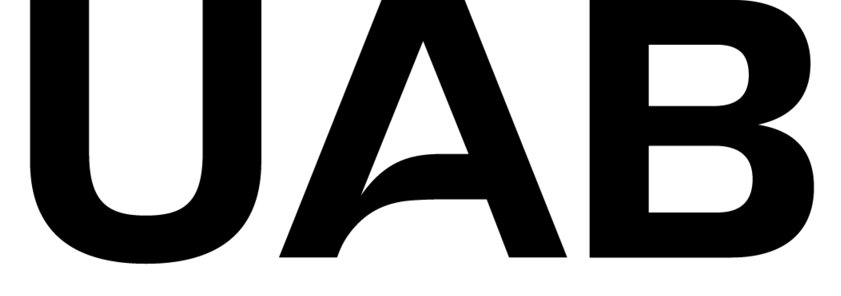
\includegraphics[width = 0.25\textwidth]{GeneralSources/UABLogo.png}\\ [0.5cm]
		\textsc{\NetIDb}\\ [2.0cm]
		\HRule{0.5pt} \\
		\LARGE \textbf{\uppercase{\documenttitle}}
		\HRule{2pt} \\ [1.5cm]
		\normalsize \begin{tabular}{rcl}  % Create a right-left column alignment
        \textsc{Author} & : & \textsc{\AuthorName} \\
        \textsc{Supervisor} & : & \textsc{Ramón Muñoz Tapia} \\
        \textsc{Co-Supervisor} & : & \textsc{Santiago Llorens Fernández}
    \end{tabular}
    \normalsize \vspace*{4.5\baselineskip}
		}

\date{2024-2025}

\author{\large \textsc{\subject} \\ \textsc{\degree}}



\begin{titlepage}
\clearpage\maketitle
\thispagestyle{empty}
\end{titlepage}

\thispagestyle{empty}
\mbox{} 
\newpage
\thispagestyle{empty}
\vspace*{\fill} % Push content to vertical center
\begin{flushright}
    \emph{Ab ovo usque ad mala.}\\[1em]
    \textbf{Horace}
\end{flushright}
\vspace*{\fill} 
\newpage
\thispagestyle{empty}
\mbox{} 
\newpage
\thispagestyle{empty}
\cfoot{}
\tableofcontents

\newpage
\pagestyle{fancyplain}
\headheight 35pt
\lhead{\NetIDb}    
\rhead{\subject}
\cfoot{\small\thepage}
\headsep 1.5em
\setcounter{page}{1}
\begin{center}
\begin{abstract}
Given a quantum state known to be prepared from an ensemble of two or more states, quantum state exclusion aims to rule out the possibility that it was prepared in a particular state from the ensemble. Using the known solution for group generated ensembles \cite{MainPaper}, we study this result as a lower bound for randomly generated ensembles via semidefinite programming.
\end{abstract}
\end{center}
%Keywords: \emph{SDP, Quantum state exclusion , \textcolor{blue}{Add keywords}}.
\section{Introduction}

\hspace{20pt}In many real-world scenarios, excluding a certain hypothesis can be more practical than solving the problem entirely. For instance, in disease diagnosis, ruling out potential illnesses is often the first step toward identifying the actual condition. Similarly, in the context of detecting a gas leak in a complex pipe system, excluding the possibility of the gas being chlorine, a toxic substance, can guide the search for the faulty pipe by narrowing down the potential sources and providing critical information about the gas's toxicity. In numerous everyday situations, the strategy of excluding specific possibilities forms a natural and often effective initial approach to the problem.

In the quantum realm, a similar line of reasoning can be applied in some problmes. One of the fundamental tasks in quantum information theory is the identification of an unknown quantum state known to belong to a given ensemble of possible states. This task is referred to as Quantum State Discrimination (\gls{qsd}), and it has been extensively studied in the literature \cite{DiscriminationArticle}. However, instead of aiming to identify the exact state, we may take another approach by applying the hypothesis exclusion idea. That is, given a quantum state known to be one among a certain ensemble, the goal becomes to conclusively rule out the possibility of the unknown state being a specific member of that ensemble. This alternative task is known as Quantum State Exclusion (\gls{qse}) \cite{PhysicsExclusionSource}, and it offers a distinct framework with its own set of advantages \cite{piani2020quantum} with respect to its counterpart \gls{qsd}.

We can approach \gls{qse} task under several protocols, depending on the context within we perform the hypothesis exclusion we can prefer one or another. In this project, we focus on two main protocols, Minimum Error (\gls{me}) and Zero Error (\gls{ze})\footnote{Also known as \emph{unambiguous exclusion}.}, i.e. the protocols for which analytical results have been presented \cite{MainPaper}. In the Minimum Error scenario, the goal is to minimize the probability of mistakenly excluding the actual prepared state. In contrast, the Zero Error approach seeks to exclude a state with absolute certainty, although this procedure sometimes yields an inconclusive result when perfect exclusion cannot be accomplished.

While \gls{qsd} has seen significant progress over the years \cite{bae2015quantum, helstromBook}, \gls{qse} has remained relatively underexplored until recently. New analytical results have emerged \cite{MainPaper} for both the \gls{me} and \gls{ze} protocols, particularly when the ensemble of quantum states possesses a certain degree of symmetry. In particular, when the ensemble is generated through the action of a finite algebraic group, the problem becomes more tractable, highlighting \gls{qse} as a worthwhile object of study.

Although the tasks of exclusion and discrimination coincide for ensembles containing only two states\footnote{Since for the two states case excluding one necessarily implies identifying the other.}, when dealing with ensembles of three or more states, the two problems diverge in both approach and complexity. Though this work primarily focuses on \gls{qse}, we include a comparative discussion of both tasks and protocols to further motivate the interest in \gls{qse} and discuss the main differences with \gls{qsd} in Appendix \ref{appendixComparisonQSDvsQSE}. One of the key features of \gls{qse} is the possibility of achieving \emph{perfect exclusion}, i.e. confidently ruling out a candidate state with complete certainty that it is not the unknown state. In contrast, \emph{perfect discrimination} is generally not achievable, meaning that one cannot identify the unknown state with absolute certainty in most settings\cite{OptimalitySRM}.

This capacity for perfect exclusion opens new avenues in quantum information theory, especially in scenarios involving partial information retrieval from quantum systems \cite{gour2020weight}. By eliminating certain hypotheses, one can extract meaningful information from a quantum system without requiring full state identification.

Building upon the recent results for the probability of a correct exclusion for group-generated ensembles \cite{MainPaper},\footnote{A proper definition of a \emph{group generated ensemble} will be given in the \emph{Group generated ensembles} section \ref{sectionGroupGeneratedEnsemble}, for the time being, we can identify them as ensembles that comprehend set of states that exhibit a certain symmetry.} this project undertakes a numerical investigation into \gls{qse}, highlighting the analytical results from group-generated ensembles as lower bounds for more general cases. The project comences with a preliminaries section that outlines the mathematical framework underlying the \gls{qse} task, along with the essential tools used in our analysis. We then present results for the probability of correct hypothesis exclusion in ensembles consisting of three quantum states, the simplest case. Furthermore, we explore the distribution of correct exclusion probabilities for randomly generated ensembles sampled according to Haar measure.\footnote{The importance of the generic ensembles generation being performed according to Haar measure is a key for the numerical analysis and it is discussed in the \emph{Methodology} section (\ref{sectionMethodology})}

To carry out our numerical analysis, we employ \gls{sdp} techniques, which allow us to cast the \gls{qse} task as a convex optimization problem. The \gls{sdp} approach has proven particularly effective for problems of this kind \cite{bandyopadhyay2014conclusive}. Finally, ve conclude by providing some theoretical intuition and insights based on our results.

\newpage
\section{Preliminaries}

\hspace{20pt}In this section we introduce some mathematical formalism of the postulates of Quantum Mechanics as well as some relevant objects in order to introduce the mathematical framework of \gls{qse} in a \gls{sdp} form. Additionally we define the Haar measure and discuss its importance for a proper generation of generic ensembles.

\subsection{Postulates and definitions}

\hspace{20pt}This project is entirely situated within the quantum realm. Therefore, we begin by contextualizing the foundational postulates, notation, and elements upon which the rest of the project relies on.

\textbf{Postulate I:} A quantum state provides a complete description of a physical system. In quantum mechanics, a state can be represented by a normalized vector $\ket{\psi}$ in a Hilbert space $\mathcal{H}$. Hence, each physical system corresponds to a unique Hilbert space.

\textbf{Postulate II:} An observable $O$ is a measurable property of a physical system. Mathematically, observables are represented by hermitian operators.

\textbf{Postulate III:} The eigenvalues $o_i$ of a hermitian operator $O = \sum_{i} o_i P_i$ represent the possible outcomes of measuring the observable $O$. Upon measuring $O$ and obtaining the result $o_i$, the quantum state $\ket{\psi}$ collapses to the state
\begin{align*}
	\frac{P_i\ket{\psi}}{\sqrt{p_i}},
\end{align*}
where $P_i$ is the projector onto the eigenspace associated with the eigenvalue $o_i$, and $p_i = \left\|P_i\ket{\psi}\right\|^2$ is the normalization factor.

\textbf{Postulate IV:} The probability $p_i$ of obtaining outcome $o_i$ when measuring the observable $O = \sum_{i} o_i P_i$ on a system described by the quantum state $\ket{\psi}$ is given by
\begin{align*}
	p_i = \text{Tr}\left(P_i \ket{\psi}\bra{\psi}\right) = \left\|P_i\ket{\psi}\right\|^2 = \braket{\psi|P_i|\psi}.
\end{align*}

%Note that if $\ket{\psi'} = e^{i\theta}\ket{\psi}$ for some global phase $\theta \in \mathbb{R}$, the observable outcomes and probabilities remain unchanged. Therefore, quantum states differing only by a global phase are physically indistinguishable.

In relation to Postulate I, it is often convenient to represent quantum states using the \emph{density matrix} formalism, where a pure  state is described by $\rho = \ket{\psi}\bra{\psi}$ instead of $\ket{\psi}$. 

%In this formalism, the global phase ambiguity disappears, since if $\ket{\psi'} = e^{i\theta}\ket{\psi}$, then
%\begin{align*}
%	\rho = \ket{\psi'}\bra{\psi'} = \ket{\psi}\bra{\psi} .
%\end{align*}

Using this representation, Postulates III and IV are reformulated. The post-measurement state has a density matrix
\begin{align*}
	\frac{P_i \rho P_i}{p_i},
\end{align*}
and the probability of obtaining outcome $o_i$ is
\begin{align*}
	p_i = \text{Tr}(P_i \rho).
\end{align*}

Both formulations are equivalent, though one may be more convenient than the other depending on the context. Furthermore, the density matrix formalism naturally introduces the concept of \emph{mixed states}. Until now, we have implicitly dealt only with \emph{pure states}, i.e., states of the form $\rho = \ket{\psi}\bra{\psi}$. Suppose now that, for reasons we ignore, the system is prepared in one of several pure states $\{\rho_i\}_{i=1}^n$ with probabilities $\{\eta_i\}_{i=1}^n$. Then the overall state of the system is described by the mixed state
\begin{align*}
	\rho = \sum_{i=1}^n \eta_i \rho_i.
\end{align*}

For the purposes of this project, we focus exclusively on pure states and do not address scenarios involving mixed states.

In relation to the observable postulate, we now define a \gls{povm} as a collection of measurement operators $\{\Pi_i\}_{i=1}^n$ that satisfy,
\begin{itemize}
	\item Each $\Pi_i$ is positive semi-definite hermitian operator, meaning all its eigenvalues $\pi_j^{(i)}$ satisfy $\pi_j^{(i)} \geq 0$.
	\item The operators satisfy the completeness relation,
\begin{align*}
	\sum_{i=1}^n \Pi_i = \mathds{1},
\end{align*}
where $\mathds{1}$ denotes the identity operator on the Hilbert space $\mathcal{H}$.
\end{itemize}

Unlike projective measurements, the operators $\Pi_i$ in a POVM are not necessarily orthogonal projectors. This allows the number of measurement outcomes to exceed the dimensionality of the Hilbert space, extending the previos orthogonal measurement to a more generic status and making POVMs particularly useful in tasks such as \gls{qse} and \gls{qsd}.

\subsection{Formulation of the problem}\label{sectionFormulationOfTheProblem}

\hspace{20pt}Let $\left\{(\rho_i, \eta_i)\right\}_{i=1}^n$ be an ensemble of $n$ quantum states, where each $\rho_i$ denotes a pure state density matrix\footnote{This formulation hols true for mixed states but the project will only discuss the pure state scenario.}, i.e., $\rho_i = \ket{\psi_i}\bra{\psi_i}$, and $\eta_i$ represents the prior probability of occurrence of the state $\rho_i$. Let $\tilde{\rho}$ be a state from this ensemble. Our objective is to develop a procedure to identify another state $\rho_j \in \left\{\rho_i\right\}_{i=1}^n$, such that $\rho_j \neq \tilde{\rho}$.

Quantum measurements are described by a set of \glspl{povm}, denoted by $\left\{\Pi_i\right\}_{i=1}^n$, acting on the Hilbert space $\mathcal{H}$ of the quantum system. Here we present the two studied protocols for \gls{qse}: minimum-error (\gls{me}) and zero-error (\gls{ze}).

As previously discussed the goal of the \gls{me} protocol is to minimize the probability of incorrectly excluding the unknown state from our hypothesis. If we formulate it as an \gls{sdp}, the \gls{sdp} minimization of the error probability reads,\footnote{Note that the \gls{sdp} formulations of quantum state discrimination may differ from the exclusion ones by interchanging minimization and maximization problems.}
\begin{align*}
	P_{\text{\gls{me}}}^e = \min_{\left\{\Pi_i\right\}} &\sum_{i=1}^n \eta_i \tr(\Pi_i \rho_i),\\
	\text{subject to} \quad & \sum_{i=1}^n \Pi_i = \mathds{1}, \quad \Pi_i \geq 0 \quad \forall i \in \{1, \dots, n\}.
\end{align*}

Note the constraints $\sum_{i=1}^n \Pi_i = \mathds{1}$ and $\Pi_i \geq 0$ ensure that the set $\{\Pi_i\}_{i=1}^n$ form a valid \gls{povm}, raising a proper probability distribution. The superscript $e$ in $P_{\text{\gls{me}}}^e$ indicates that this is the \emph{error probability}.

Alternatively, we may formulate the problem in terms of the \emph{success probability}, denoted by $P_{\text{\gls{me}}}^s$, which quantifies the probability of a correct exclusion. This equivalent formulation reads,
\begin{align*}
	P_{\text{\gls{me}}}^s = \max_{\left\{\Pi_i\right\}} &\left(1 - \sum_{i=1}^n \eta_i\tr(\Pi_i \rho_i)\right),\\
	\text{subject to} \quad & \sum_{i=1}^n \Pi_i = \mathds{1}, \quad \Pi_i \geq 0 \quad \forall i \in \{1, \dots, n\}.
\end{align*}

Naturally, both formulations are related via,
\begin{align*}
P_{\text{\gls{me}}}^s + P_{\text{\gls{me}}}^e = 1.
\end{align*}

In the case of the \gls{ze} protocol, the objective is to exclude with total accuracy a state known to be different from the unkown state. However, the protocol might lead to inconclusive result. In order to do so, the \gls{povm}s must also satisfy an unambiguity condition, i.e. each measurement operator $\Pi_i$ must be orthogonal to the corresponding state $\rho_i$. In other words,
\begin{align*}
\tr(\Pi_i \rho_i) = 0 \quad \forall i \in \{1, \dots, n\}.
\end{align*}

To ensure completeness, we introduce an additional \gls{povm} element $\Pi_?$ representing an inconclusive result,
\begin{align*}
\Pi_? = \mathds{1} - \sum_{i=1}^n \Pi_i.
\end{align*}

If the measurement yields the outcome $\Pi_?$, i.e., the "?" label, the result is inconclusive.

The corresponding \gls{sdp} for minimizing the probability of an inconclusive result, i.e. error, in the \gls{ze} protocol is,
\begin{align*}
	P_{\text{\gls{ze}}}^e = \min_{\left\{\Pi_i\right\}} &\sum_{i=1}^n \eta_i\tr(\Pi_? \rho_i),\\
	\text{subject to} \quad & \sum_{i=1}^n \Pi_i + \Pi_? = \mathds{1}, \quad \Pi_? \geq 0,\\
	& \tr(\Pi_i \rho_i) = 0, \quad \Pi_i \geq 0 \quad \forall i.
\end{align*}

The corresponding success probability is naturally given by, the maximization of $1-P_{\text{\gls{ze}}}^e$ under the same constraints.

Notice this formulation is analogous to the \gls{me} protocol, with the crucial difference being the constraint $\tr(\Pi_i \rho_i) = 0$, enforcing unambiguous discrimination.

Additionally, in some cases it is useful to consider the dual formulation of the problem, as solving the dual version of the \gls{sdp} can often be more computationally efficient. Moreover, one may consider an ansatz, i.e. a candidate set of \gls{povm}s, and compute the exclusion success probability under a given protocol. This provides a lower bound for the success probability, since in principle we cannot guarantee that this ansatz is optimal, i.e. there may exist another set of \gls{povm}s yielding a higher success rate.

However, by evaluating the same set of \gls{povm}s within the dual formulation, we can obtain an upper bound on the success probability. If the upper and lower bounds coincide, we can conclude that the chosen \gls{povm} set is indeed optimal. For this reason, we present the dual formulation of the problem in Appendix~\ref{sectionDualFormulationOfTheProblem}. This procedure is standard for verifying the optimality of a given \gls{povm} set and closely resembles the internal computations performed by a \gls{sdp} solver.

\subsection{Gram Matrix Formulation}\label{sectionGramMatrixFormulation}
\hspace{20pt}The Gram matrix formulation recasts the \gls{sdp} problems associated with the exclusion task in a more basis-independent manner. This approach reveals that the exclusion tasks for certain ensembles can be equivalent to those of others. As such, we adopt this formulation in our analysis, as it offers valuable insight into the underlying relationships between the quantum states in the ensemble.

Given an ensemble $\left\{(\rho_i, \eta_i)\right\}_{i=1}^n$ of $n$ quantum states we define the $\mathcal{G} \in \mathbb{C}^{n \times n}$ be the \emph{Gram matrix} of the ensemble, as the $n \times n$ positive semidefinite Hermitian matrix given by,
\begin{equation*}
	\mathcal{G} =
	\begin{pmatrix}
		\eta_1 & \sqrt{\eta_1\eta_2}\braket{\psi_1|\psi_2} & \dots & \sqrt{\eta_1\eta_n}\braket{\psi_1|\psi_n} \\
		\sqrt{\eta_2\eta_1}\braket{\psi_2|\psi_1} & \eta_2 & \dots & \sqrt{\eta_2\eta_n}\braket{\psi_2|\psi_n} \\
		\vdots & \vdots & \ddots & \vdots \\
		\sqrt{\eta_n\eta_1}\braket{\psi_n|\psi_1} & \sqrt{\eta_n\eta_2}\braket{\psi_n|\psi_2} & \dots & \eta_n
	\end{pmatrix},
\end{equation*}

that is, $\mathcal{G}_{i,j} = \sqrt{\eta_i\eta_j}\braket{\psi_i|\psi_j}$. Since all states are normalized, the diagonal elements are equal to $\eta_i$.

By construction, the Gram matrix is Hermitian,
\begin{align*}
	\mathcal{G}_{i,j}^* = \left( \sqrt{\eta_i\eta_j}\braket{\psi_i|\psi_j}\right)^* =  \sqrt{\eta_j\eta_i}\braket{\psi_j|\psi_i} = \mathcal{G}_{j,i}.
\end{align*}
Additionally, $\mathcal{G}$ is positive semidefinite. To see this, consider an arbitrary state $\ket{\Phi}$ and an orthonormal basis $\{\ket{i}\}_{i=1}^n$, then,
\begin{align*}
	\braket{\Phi|\mathcal{G}|\Phi} &= \braket{\Phi| \left( \sum_{i,j=1}^{n} \sqrt{\eta_i\eta_j}\braket{\psi_i|\psi_j} \ket{i}\bra{j} \right) |\Phi} \\
	&= \sum_{i,j=1}^{n} \sqrt{\eta_i\eta_j}\braket{\psi_i|\psi_j} \braket{\Phi|i} \braket{j|\Phi} \\
	&= \left\| \sum_{i=1}^{n} \eta_i\braket{i|\Phi} \ket{\psi_i} \right\|\\
	&\geq 0.
\end{align*}

Since $\mathcal{G}$ is Hermitian and positive semidefinite, it can be factorized as,

\begin{align*}
	\mathcal{G} = X^\dagger X,
\end{align*}

for some matrix $X$, whose columns are the pure states,

\begin{align*}
	X = \begin{pmatrix}
		\mid & \mid &        & \mid \\
		\sqrt{\eta_i}\ket{\psi_1} & \sqrt{\eta_2}\ket{\psi_2} & \dots & \sqrt{\eta_n}\ket{\psi_n} \\
		\mid & \mid &        & \mid
	\end{pmatrix}.
\end{align*}

Let us fix an arbitrary orthonormal basis $\{\ket{\omega_i}\}_{i=1}^n$. Then, the diagonal entries of $X$ in this basis are given by,
\begin{align*}
	X_{i,i} = \sqrt{\eta_i}\braket{\omega_i|\psi_i}.
\end{align*}
\footnote{Note that fixing the basis $\{\ket{\omega_i}\}_{i=1}^n$ uniquely determines the decomposition $\mathcal{G} = X^\dagger X$, and vice versa.}We define the POVM elements as projectors $\Pi_i = \ket{\omega_i}\bra{\omega_i}$. Then, for the ensemble $\{(\rho_i, \eta_i)\}_{i=1}^n$, the corresponding semidefinite program (\gls{sdp}) constrains become,
\begin{align*}
	\eta_i\tr(\Pi_i \rho_i) &= \eta_i\tr\left( \ket{\omega_i}\bra{\omega_i} \ket{\psi_i}\bra{\psi_i} \right) \\
	&= |\sqrt{\eta_i}\braket{\omega_i|\psi_i}|^2 \\
	&= |X_{i,i}|^2.
\end{align*}

Thus, we can reformulate the \gls{sdp} for the minimum-error (\gls{me}) protocol as,
\begin{align*}
	P_{\gls{me}}^e = \min_{X} &\sum_{i=1}^n |X_{i,i}|^2, \\
	\text{subject to} \quad & X^\dagger X = \mathcal{G}, \quad X \geq 0.
\end{align*}

Similarly, the success probability becomes,
\begin{align*}
	P_{\gls{me}}^s = \max_{X} &\left( 1 - \sum_{i=1}^n |X_{i,i}|^2 \right), \\
	\text{subject to} \quad & X^\dagger X = \mathcal{G}, \quad X \geq 0.
\end{align*}

This reformulation reveals that if two ensembles $A$ and $B$ share the same Gram matrix, then their exclusion problems under both the \gls{me} and \gls{ze} protocols are equivalent. That is, their optimal success and error probabilities coincide. Consequently, we focus on the Gram matrix to study exclusion problems rather than the explicit state representations.

%Furthermore, we note that the case of arbitrary prior probabilities $\eta_i$ can be reduced to the equal prior case $\eta_i = \frac{1}{n}$ by defining non-normalized states,
%\begin{align*}
%	\ket{\tilde{\psi}_i} = \frac{1}{\sqrt{\eta_i}} \ket{\psi_i},
%\end{align*}
%and reformulating the problem in terms of these states. The prior probabilities are then absorbed into the state norm. 

\subsection{Group Generated Ensembles}\label{sectionGroupGeneratedEnsemble}

\hspace{20pt}As we have mentioned before, analytical results have been found for the exclusion task in both protocols \gls{me} and \gls{ze} for ensembles that exhibit a certain degree of symmetry\cite{MainPaper}, that is for \emph{group-generated} ensembles. In this section we present a proper definition for a group-generated ensemble as well as a brief discussion on this ensembles generated by a cyclic group, a key type of grop-generated ensembles in our analysis.

Given a quantum state $\ket{\psi}$, referred to as the \emph{seed state}, we define a \emph{group generated ensemble} as the set of states obtained by applying a group of unitary transformations to $\ket{\psi}$. Specifically, if the ensemble consists of $n$ quantum states, its elements are of the form,

\begin{align*}
	U_i\ket{\psi}, \quad i \in \{1, \dots, n\},
\end{align*}

where the set of unitary matrices $\{U_i\}_{i=1}^n$ forms a finite group under standard matrix multiplication. In terms of density matrices, the ensemble can equivalently be written as,

\begin{align*}
	\rho_i = U_i \rho U_i^\dagger, \quad i \in \{1, \dots, n\},
\end{align*}

where $\rho = \ket{\psi}\bra{\psi}$ is the density matrix corresponding to the seed state.

For instance, let $\mathcal{U}$ be a unitary operator such that $\mathcal{U}^n = \mathds{1}$ (i.e., $\mathcal{U}$ generates a cyclic group of order $n$). Then, the set of states
\begin{align*}
	\left\{ \mathcal{U}^i\ket{\psi} \right\}_{i=0}^{n-1},
\end{align*}

forms a group generated ensemble based on the cyclic group $\mathbb{Z}/n\mathbb{Z}$. This type of ensemble is of particular interest in our study and will be explored in more detail at the end of this section. Additionally, in Appendix \ref{appendixComputationGroupGeneratedGramMatrices} we present a general procedure to compute the Gram Matrix for any group-generated ensemble.

\subsubsection*{The $\mathbb{Z}/n\mathbb{Z}$ group-generated ensemble}

\hspace{20pt}Here we discuss the particular case for a $\mathbb{Z}/n\mathbb{Z}$ group-generated ensemble a key type of ensemble for our project.\footnote{The relevance of this type of ensembles relies on the fact that for a prime number of states, the possible group-generated group ensemble } Let $\mathcal{U} \in U(n)$ be an $n \times n$ unitary matrix satisfying $\mathcal{U}^n = \mathds{1}$, and let $\ket{\psi}$ be the seed state. The Gram matrix $\mathcal{G}^{\mathbb{Z}/n\mathbb{Z}}$ elements associated with the ensemble $\left\{\mathcal{U}^i\ket{\psi}\right\}_{i=0}^{n-1}$ are,
\begin{align*}
	\mathcal{G}^{\mathbb{Z}/n\mathbb{Z}}_{i,j} = \sqrt{\eta_i \eta_j}\braket{\mathcal{U}^i\psi | \mathcal{U}^j\psi} = \sqrt{\eta_i \eta_j}\braket{\psi | \mathcal{U}^{j-i} | \psi} = \sqrt{\eta_i \eta_j}\braket{\mathcal{U}^{j-i}}_{\psi},
\end{align*}

where we use the shorthand notation,
\begin{align*}
	\braket{\mathcal{U}^k}_\psi := \braket{\psi | \mathcal{U}^k | \psi}.
\end{align*}

Using this, the Gram matrix $\mathcal{G}^{\mathbb{Z}/n\mathbb{Z}}$ can be expressed as a circulant matrix,
\begin{align*}
	\mathcal{G}^{\mathbb{Z}/n\mathbb{Z}} = \begin{pmatrix}
 \eta_1 & \sqrt{\eta_1 \eta_2}\braket{\mathcal{U}}_{\psi} & \sqrt{\eta_1 \eta_3}\braket{\mathcal{U}^2}_{\psi} & \cdots & \sqrt{\eta_1 \eta_n}\braket{\mathcal{U}^{n-1}}_{\psi} \\
 \sqrt{\eta_2 \eta_1}\braket{\mathcal{U}^{n-1}}_{\psi}^* & \eta_2 & \sqrt{\eta_2 \eta_3}\braket{\mathcal{U}}_{\psi} & \cdots & \sqrt{\eta_2 \eta_n}\braket{\mathcal{U}^{n-2}}_{\psi} \\
 \sqrt{\eta_1 \eta_3}\braket{\mathcal{U}^{n-2}}_{\psi}^* & \sqrt{\eta_2 \eta_3}\braket{\mathcal{U}^{n-1}}_{\psi}^* & \eta_3 & \cdots & \sqrt{\eta_3 \eta_n}\braket{\mathcal{U}^{n-3}}_{\psi} \\
 \vdots & \vdots & \vdots & \ddots & \vdots \\
 \sqrt{\eta_1 \eta_n}\braket{\mathcal{U}}_{\psi} & \sqrt{\eta_2 \eta_n}\braket{\mathcal{U}^{2}}_{\psi} & \sqrt{\eta_3 \eta_n}\braket{\mathcal{U}^{3}}_{\psi} & \cdots & \eta_n
\end{pmatrix}.
\end{align*}

Note that the Gram matrix is Hermitian, as expected, since
\begin{align*}
    \braket{\mathcal{U}^{-j}}_{\psi} = \braket{\psi | \mathcal{U}^{-j} | \psi} = \left(\braket{\psi | \mathcal{U}^j | \psi}\right)^* = \braket{\mathcal{U}^j}_{\psi}^*.
\end{align*}

Additionally, by using the identity $\mathcal{U}^n = \mathds{1}$, we can simplify expressions such as,
\begin{align*}
	\braket{\mathcal{U}^{-n+i}}_\psi = \braket{\psi | \mathcal{U}^{-n+i} | \psi} = \braket{\psi | \mathcal{U}^i | \psi} = \braket{\mathcal{U}^i}_\psi.
\end{align*}

Thus, we may write,
\begin{align*}
	\mathcal{G}^{\mathbb{Z}/n\mathbb{Z}} = \begin{pmatrix}
 \eta_1 & \sqrt{\eta_1 \eta_2}\braket{\mathcal{U}}_{\psi} & \sqrt{\eta_1 \eta_3}\braket{\mathcal{U}^2}_{\psi} & \cdots & \sqrt{\eta_1 \eta_n}\braket{\mathcal{U}}^*_{\psi} \\
 \sqrt{\eta_2 \eta_1}\braket{\mathcal{U}}^*_{\psi} & \eta_2 & \sqrt{\eta_2 \eta_3}\braket{\mathcal{U}}_{\psi} & \cdots & \sqrt{\eta_2 \eta_n}\braket{\mathcal{U}}^*_{\psi} \\
 \sqrt{\eta_1 \eta_3}\braket{\mathcal{U}^2}^*_{\psi} & \sqrt{\eta_2 \eta_3}\braket{\mathcal{U}}^*_{\psi} & \eta_3 & \cdots & \sqrt{\eta_3 \eta_n}\braket{\mathcal{U}}^*_{\psi} \\
 \vdots & \vdots & \vdots & \ddots & \vdots \\
 \sqrt{\eta_1 \eta_n}\braket{\mathcal{U}}_{\psi} & \sqrt{\eta_2 \eta_n}\braket{\mathcal{U}^{2}}_{\psi} & \sqrt{\eta_3 \eta_n}\braket{\mathcal{U}^{3}}_{\psi} & \cdots & \eta_n
\end{pmatrix}.
\end{align*}

This shows the circulant structure of $\mathcal{G}$ for a equal prior probability case, where each row is a cyclic permutation of the previous one. In other words, the Gram matrices of $\mathbb{Z}/n\mathbb{Z}$-generated ensembles are circulant matrices when taking equal priors probabilities. This structure is particularly useful, as circulant matrices can be diagonalized by the discrete Fourier basis, greatly simplifying many computations~\cite{circulantMatrices}.

The Fourier basis for an $n \times n$ circulant matrix consists of the set of vectors $\{\omega_i\}_{i=1}^n$, where
\begin{align*}
	\omega_i = \frac{1}{\sqrt{n}} (1, \gamma^i, \gamma^{2i}, \ldots, \gamma^{i(n-1)})^T,
\end{align*}

and
\begin{align*}
	\gamma = e^{\frac{2\pi i}{n}}.
\end{align*}

Finally, we denote the cardinality of a finite group $G$, i.e. the number of its elements of the group, as $|G|$. In scenarios with uniform prior probabilities, this implies,
\begin{align*}
	\eta_i = \frac{1}{|G|}\quad \forall i\in\{1,...,n\}.
\end{align*}
\subsection{Previous Results}\label{sectionPreviousResults}

\hspace{20pt}Significant progress has been made in the study of the state exclusion task for group-generated ensembles. In particular, the work \emph{Quantum State Exclusion for Group-Generated Ensembles of Pure States}\cite{MainPaper} presents exact analytical expressions for the success and error probabilities under both the Minimum Error (\gls{me}) and Zero Error (\gls{ze}) exclusion protocols. In this section we present this results and comment some key aspects of this results regarding our project, in particular we present the concept of \emph{perfect exclusion region} and we discuss the case of ensembles with a prime number of states.

Let $\mathcal{G}^G$ denote the Gram matrix of a group-generated ensemble $\left\{ \left( \rho_i, \frac{1}{|G|} \right) \right\}_{i=1}^{|G|}$, where $G$ is a finite group of size $|G|$, and let $\{\lambda_i\}_{i=1}^{|G|}$ be the set of eigenvalues of $\mathcal{G}^G$, the Gram Matrix of the group. Assume the eigenvalues $\left\{\frac{\lambda_i}{|G|}|1\leq i \leq n\right\}$ are ordered increasingly,
\begin{align*}
	i \leq j \quad \Leftrightarrow \quad \lambda_i \leq \lambda_j, \quad \forall i,j \in \{1, \dots, |G|\},
\end{align*}

i.e., $\frac{\lambda_1}{|G|}$ is the smallest and $\lambda_{|G|}$ the largest eigenvalue. Notice that since we are in the equal probability scenario, we can factor out a $\frac{1}{|G|}$ factor from the Gram Matrix and consider the matrix $|G|\mathcal{G}^G$ instead of $\mathcal{G}^G$, i.e. the eigenvalues of this matrix simply are $\left\{\lambda_i\right\}_{i=1}^n$. This is a standard choice for simplicity, when we dealing with equal prior probabilities.

The exclusion probabilities under the Minimum Error protocol are given by,
\begin{align*}
	P_{\gls{me}}^e &= \max\left\{ 0, \left( \frac{ \sqrt{\lambda_{|G|}} - \sum_{i<|G|} \sqrt{\lambda_i} }{|G|} \right)^2 \right\}, \\
	P_{\gls{me}}^s &= \min\left\{ 1, 1 - \left( \frac{ \sqrt{\lambda_{|G|}} - \sum_{i<|G|} \sqrt{\lambda_i} }{|G|} \right)^2 \right\}.
\end{align*}

For the Zero Error protocol, the corresponding expressions arem
\begin{align*}
	P_{\gls{ze}}^e &= \max\left\{ 0, \frac{ \sum_{i=1}^{|G|} \sqrt{\lambda_i} \left( \sqrt{\lambda_{|G|}} - \sum_{j<|G|} \sqrt{\lambda_j} \right) }{|G|} \right\}, \\
	P_{\gls{ze}}^s &= \min\left\{ 1, 1 - \frac{ \sum_{i=1}^{|G|} \sqrt{\lambda_i} \left( \sqrt{\lambda_{|G|}} - \sum_{j<|G|} \sqrt{\lambda_j} \right) }{|G|} \right\}.
\end{align*}

A key feature of these results is their independence from the specific group generating the ensemble. That is, for any two group-generated ensembles $A$ and $B$ corresponding to groups $G_A$ and $G_B$, with $G_A \neq G_B$ but $|G_A| = |G_B|$, if their respective Gram matrices $\mathcal{G}^{G_A}$ and $\mathcal{G}^{G_B}$ share the same eigenvalues, then the exclusion probabilities for both \gls{me} and \gls{ze} protocols are identical. This group-independence property is a cornerstone of the present study.

Another important outcome from \cite{MainPaper} is the identification of conditions under which perfect exclusion is achievable, i.e., the exclusion can be carried out with zero error. This occurs if the eigenvalues satisfy the inequality,

\begin{align}\label{equationPerfectExclusionCondition}
	\lambda_{|G|} \leq \left( \sum_{i<|G|} \sqrt{\lambda_i} \right)^2.
\end{align}

We refer to the regime satisfying this inequality as the \emph{perfect exclusion zone}. Within this regime, the success probability of the exclusion task reaches one, implying that exclusion can be performed perfectly.

In this project, we will extend this result by demonstrating that the perfect exclusion condition Eq. (\ref{equationPerfectExclusionCondition}) provides a lower bound for the success probability of exclusion even for non-group-generated ensembles. Since this bound equals 1, it implies that any ensemble whether or not group-generated that satisfies condition Eq. (\ref{equationPerfectExclusionCondition}) can achieve perfect exclusion. Thus, the perfect exclusion zone is not exclusive to group-generated ensembles, but also includes all ensembles that fulfill the given condition.

Furthermore, we might highlight a key aspect of the analytical solutions for the \gls{qse} task form \gls{me} and \gls{ze} protocols. These results depend solely on the eigenvalues of the Gram matrix and are independent of the specific group structure generating the ensemble. Hence, let the Gram matrix of an ensemble decompose as,
\begin{align*}
	\mathcal{G} = U D U^\dagger,
\end{align*}

where $U$ is a unitary matrix and $D$ is the diagonal matrix of eigenvalues. We then encounter two possibilities,
\begin{itemize}
	\item The eigenvalues satisfy Eq.~\eqref{equationPerfectExclusionCondition}, placing the ensemble in the \emph{perfect exclusion} regime.
	\item The eigenvalues do not satisfy Eq.~\eqref{equationPerfectExclusionCondition}, placing the ensemble in the \emph{non-perfect exclusion} regime.
\end{itemize}

In the perfect exclusion regime, the existence of a \gls{povm}, such that the measurement outcome allows exclusion of a hypothesis without error, is guaranteed.

In the non-perfect exclusion regime, the analytical results for group-generated ensembles provide lower bounds on the success probabilities, and upper bounds on the error probabilities for general ensembles.

Consider, for example, the case of an ensemble of 4 quantum states. There are exactly two groups of four elements, $\mathbb{Z}/4\mathbb{Z}$ and $\mathbb{Z}/2\mathbb{Z} \times \mathbb{Z}/2\mathbb{Z}$.\footnote{These are the only non-isomorphic groups of order 4.} This implies that there exist two specific unitary matrices, $U_{\mathbb{Z}/4\mathbb{Z}}$ and $U_{\mathbb{Z}/2\mathbb{Z} \times \mathbb{Z}/2\mathbb{Z}}$ (up to permutation of rows and columns), for which the analytical solution holds exactly.

Since $U(n)$ is compact, and assuming continuity of the exclusion probabilities with respect to $U$ under a given matrix norm, for each of these unitary matrices there exist arbitrarily small neighborhoods $\mathcal{B}(U_{\mathbb{Z}/4\mathbb{Z}})$ and $\mathcal{B}(U_{\mathbb{Z}/2\mathbb{Z} \times \mathbb{Z}/2\mathbb{Z}})$ such that the exclusion probabilities within these neighborhoods approximate the analytical result as closely as desired. However, the existence of multiple such matrices, and intersecting neighborhoods, can complicate numerical optimization and analysis.

In contrast, it is usefull to consider the case where the ensemble contains a prime number $p$ of states. In this scenario, the situation simplifies considerably, since there exists only one group, up to isomorphism, of order $p$, namely $\mathbb{Z}/p\mathbb{Z}$.

This result follows immediately from Lagrange's theorem. The theorem guarantees the order of any element in a finite group\footnote{The order of an element $\tau$ in a group $G$ is the smallest positive integer $m$ such that $\tau^m = e$, where $e$ denotes the identity/neutral element of the group.} must divide the order of the group. Since $p$ is a prime number, the only positive integers dividing $p$ are either $1$ or $p$ itself. Therefore, the order of any group element must be either $1$ or $p$. An element of order $1$ must be the identity, so every non-identity element in the group must have order $p$. This implies that all non-identity elements generate the entire group, i.e., the group is cyclic. As a result, any group of prime order $p$ is necessarily cyclic and isomorphic to $\mathbb{Z}/p\mathbb{Z}$.

Consequently, for an ensemble of $p$ quantum states, there exists a unique unitary matrix $U_{\mathbb{Z}/p\mathbb{Z}}$ (up to reordering) that diagonalizes the Gram matrix in such a way that the analytical results are exact. \footnote{Moreover, the columns of this matrix correspond to the elements of the Fourier basis, as discussed in Section~\ref{sectionGroupGeneratedEnsemble}, particularly in the example involving $\mathbb{Z}/n\mathbb{Z}$.}

Ensembles containing a prime number of states are of particular interest, as the analytical result can be guaranteed to be exact for only one specific ensemble. Consequently, when interpreting the results for the case of generic ensembles in the following sections we can be ensure the analytical result is exact in only one instance. Moreover, there is no overlap with other Gram matrices for which the result would also hold exactly.

\subsection{Haar Measure}
\hspace{20pt}In this section, we introduce the concept of a measure on a topological space and define the Haar measure. This is one of the key theoretical tools underlying this project, as we use the Haar measure to ensure a uniform and unbiased sampling of ensembles when generating Gram matrices for general ensembles.

Let \( \Omega \) be a set, and let \( \Sigma \) be a \( \sigma \)-algebra over \( \Omega \). A measure \( \mu \) on the measurable space \( (\Omega, \Sigma) \) is a set function \( \mu : \Sigma \to \mathbb{R}_{\geq 0} \) that satisfies the following properties:
\begin{itemize}
	\item Positive semidefiniteness, i.e. for any $\chi\in\Sigma$ we have $\mu(\chi)\geq 0$.
	\item $\mu(\emptyset)=0$.
	\item Sigma additivity, i.e. given a countable set $\{\chi_i\in\Sigma|i\in\mathbb{N}\}$ of pairwise-disjoint sets\footnote{This means that $\chi_i\cap\chi_j=\emptyset$ for any $i,j\in\mathbb{N}$ if $i\neq j$.} $\mu$ fulfils, 
	\begin{align*}
		\mu\left(\bigcup_{i=1}^\infty \chi_i\right)=\sum_{i=1}^\infty \mu(\chi_i).
	\end{align*}
\end{itemize}

Now, let \( \Omega \) be a topological group. A Haaar measure \( \mu \) on a set \( \Omega \) is a measure defined on the Borel \( \sigma \)-algebra \( \Upsilon \) of \( \Omega \)\footnote{A full definition of Borel sets is beyond the scope of this work, it is enough to say they are sets generated from the open sets of \( \Omega \) through countable unions, intersections, and complements.}, satisfying the following properties:
\begin{itemize}
	\item Invariance under transition, i.e. for any $\omega \in \Omega$ and $\upsilon \in \Upsilon$ we have $\mu(\omega\upsilon)=\mu(\upsilon)$.
	\item The measure is finite for any compact Borel subset, i.e. for any $\upsilon\in\Upsilon$ compact we have that $\mu(\upsilon)<\infty$.
	\item $\mu$ is outer regular, i.e. for any $\upsilon\in\Upsilon$
		\begin{align*}
			\mu(\upsilon)=\inf_{\vartheta\:\text{open}}\{\mu(\vartheta)|\upsilon\subseteq\vartheta\}
		\end{align*}
	\item $\mu$ is inner regular, i.e. for any open $\upsilon\in\Upsilon$,
		\begin{align*}
			\mu(\upsilon)=\sup_{\vartheta\:\text{compact}}\{\mu(\vartheta)|\vartheta\subseteq\upsilon\}
		\end{align*}
\end{itemize}

It can be shown that the Haar measure is unique up to a constant multiple. In particular, since we are working with the set of unitary matrices,
\begin{align*}
	U(n) = \{ U \in \mathbb{C}^{n \times n} \mid U^\dagger U = \mathds{1} \},
\end{align*}

which is compact in the usual topology, from the secon property we know the Haar measure \( \mu \) on \( U(n) \) to be finite. Therefore, we can normalize it so that \( \mu(U(n)) = 1 \), fully determining the measure. Moreover, since from the first property we know \( \mu \) is invariant under group multiplication, it is uniformly distributed over \( U(n) \). This allows us to generate unitary matrices that are randomly and uniformly distributed with respect to the Haar measure.

\newpage
\section{Methodology}\label{sectionMethodology}

\hspace{20pt}All the used code in this project is hosted in the GitHub repository \cite{GitHub}, where additional documentation is available detailing the functionality and structure of each script and class involved in the implementation. The numerical analysis is performed by generating ensembles uniformly distributed taking into account all possibilities and then solving the \gls{sdp} problems presented in Section \ref{sectionFormulationOfTheProblem}.

The core of the numerical analysis is the implementation of a Semi-Definite Programming (\gls{sdp}) solver based on the MOSEK optimization suite \cite{mosek_sdp}, interfaced through the Python-based PICOS optimization library \cite{PICOS}. 

To analyze both group-generated and generic quantum state ensembles, we developed a method for generating random Gram matrices with prescribed spectral properties.

A Numpy \gls{rng}\cite{numpyRNG} produces a set of $n$ non-negative real numbers $\{\lambda_i\}_{i=1}^n$ that are normalized to satisfy the trace condition,
\begin{align*}
	\sum_{i=1}^n \lambda_i = 1.
\end{align*}

These values are used as the eigenvalues of the Gram matrix, forming the diagonal matrix $D = \operatorname{diag}(\lambda_1, \dots, \lambda_n)$. 

Next, we generate a unitary matrix $U$ and construct the Gram matrix as,
\begin{align*}
	\mathcal{G} = U D U^\dagger.
\end{align*}

At this point, we choose whether the ensemble is to be group-generated or generic.

For a generic ensemble, the unitary matrix $U$ is drawn randomly according to the Haar measure \cite{haarMeasure}, which defines the unique uniform probability measure on the unitary group $U(n)$ that is invariant under group multiplication. To ensure this uniformity, we use the algorithm introduced by Francesco Mezzadri in \cite{UnitaryMatricesGeneration}, which provides an efficient and accurate way of sampling unitary matrices while uniformly covering $U(n)$. 

This aspect is crucial: if the random generation of unitary matrices did not uniformly cover U(n), the numerical analysis would be fundamentally flawed. It would lead to an overrepresentation of certain types of ensembles, potentially missing rare or atypical configurations. As a result, ensembles that might violate the theoretical lower bound could be systematically avoided, rendering the conclusions of the analysis unreliable.

In the case of a group-generated ensemble, we restrict ourselves to ensembles generated by the cyclic group $\mathbb{Z}/n\mathbb{Z}$. The corresponding unitary matrix $U$ is constructed such that its columns are the vectors of the discrete Fourier basis, as discussed in Section~\ref{sectionGroupGeneratedEnsemble} (\emph{Group-Generated Ensemble}).

Other groups are omitted in our analysis since we can always choose $n$ to be a prime number, in which case the only group of order $n$ (up to isomorphism) is the cyclic group $\mathbb{Z}/n\mathbb{Z}$. This significantly simplifies the group structure and ensures that the only group-generated ensemble under consideration corresponds to a well-defined, unique construction.

This methodology provides a flexible yet rigorous foundation for both exploring generic quantum ensembles and benchmarking them against analytically tractable group-generated cases.

\newpage
\section{Results and Discussion}\label{sectionResultsAndDiscussion}

\hspace{20pt}The begining of the analysis consists in showing up the key differences between \gls{me} and \gls{ze} protocols, and the concordance of the \gls{sdp}'s numerical results with the analytical results given in \ref{sectionPreviousResults}.

The case of ensembles conformed by 3 states is one of the main objects of study, that is because it is the only ensemble that we can entirely represent 2 dimensional plots with. In orther to show up this fact, let us analyze the case of a $\mathbb{Z}/3\mathbb{Z}$ ensemble for equal priors probabilities. The Gram matrix in this case takes the form,

\begin{align*}
	\mathcal{G}^{\mathbb{Z}/3\mathbb{Z}}=\frac{1}{3}\begin{pmatrix}
		1 & c & c^*\\
		c^* & 1 & c\\
		c & c^* & 1
	\end{pmatrix}
\end{align*}

with $c \in \mathbb{C}$. Note that, with respect to previous notation, we write $c = \braket{U}_{\psi}$, where $c$ and $c^*$ denote the overlap between different states. We can parametrize $c$ as $c = |c|e^{i\phi}$, and since we are analyzing normalized states,
\begin{align*}
	|c|\in [0,1], \quad \phi\in[0,2\pi]
\end{align*}
we observe two \gls{dof}.

Since 3 is a prime number, the only group of order 3 is $\mathbb{Z}/3\mathbb{Z}$, as discussed in Section (\ref{sectionLimitCaseScenarios}). The Gram matrix can be diagonalized as,
\begin{align*}
	\mathcal{G}^{\mathbb{Z}/3\mathbb{Z}} = U_{\mathbb{Z}/3\mathbb{Z}} D U_{\mathbb{Z}/3\mathbb{Z}}^\dagger,
\end{align*}
where $U_{\mathbb{Z}/3\mathbb{Z}}$ is the unitary matrix with Fourier basis vectors as columns. The eigenvalues of the simplified matrix, i.e. $3\mathcal{G}^{\mathbb{Z}/3\mathbb{Z}}$ matrix are denoted as $\{\lambda_1,\lambda_2,\lambda_3\}$ with $\lambda_1 \leq \lambda_2 \leq \lambda_3$. Since,
\begin{align*}
	\sum_{i=1}^3 \lambda_i = 3
\end{align*}

we again find only two \glspl{dof}, consistent with our earlier parameterization. Furthermore, since $\mathcal{G}^{\mathbb{Z}/3\mathbb{Z}} \geq 0$, we have,

\begin{align*}
	\lambda_i \geq 0 \quad \forall i \in \{1,2,3\},
\end{align*}
implying the eigenvalues must lie in the interval $[0,3]$.\footnote{In general, eigenvalues lie in $[0,n]$ for an $n$-dimensional ensemble, even for non-group-generated ensembles.} Therefore,
\begin{align*}
	\lambda_3 \in [0,3], \quad \lambda_2 \in [0,\lambda_3], \quad \lambda_1 = 3 - \lambda_2 - \lambda_3.
\end{align*}

This scenario is particularly interesting as it is the only ensemble with a small enough dimension to fully visualize all parameter dependencies and study the ensemble structure.\footnote{Visualizations include two parameters along with the success/exclusion probability of the respective protocol.} Higher-dimensional cases are too complex for full representation, while two-state cases reduce to standard quantum state discrimination (\gls{qsd}) as previously discussed.

\subsection{Comparison \gls{me} vs. \gls{ze}}

\hspace{20pt}Here we present a comparison between both protocols for \gls{ze} and \gls{me} giving insights on the protocols's essence and contextualising the problem in a visual way.

In Figure (\ref{FigureQSEMEZ3ZHeatmap})  we presents the \gls{me} (left) and \gls{ze} (right) protocols results for the \gls{qse} task. In particular Figure (\ref{FigureQSEMEZ3ZHeatmap}) shows two heatmaps of the average successful exclusion probability under the Minimum Error (\gls{me}) protocol for a $\mathbb{Z}/3\mathbb{Z}$ group-generated ensemble. Probabilities are shown as functions of the modulus $|c|$ ($x$-axis) and phase $\theta$ ($y$-axis) of the overlap $c=|c|^{i\theta}$, which fully determines the Gram matrix. Notice we take equal prior probabilities, as discussed in the analytical results in Section (\ref{sectionPreviousResults}). 

\begin{figure}[H]
	\centering
	\begin{overpic}[width=0.49\textwidth, trim={2.3cm 0.8cm 4.3cm 2cm}, clip]{../Plots/ExlusionOverlapVSPhaseVSMinimumErrorProbabilityZ3HeatMap.pdf}
		\put(60,25){$\mathcal{G}^{\mathbb{Z}/3\mathbb{Z}}<0$}
		\put(60,55){$\mathcal{G}^{\mathbb{Z}/3\mathbb{Z}}<0$}
	\end{overpic}
		\begin{overpic}[width=0.49\textwidth, trim={2.3cm 0.8cm 4.5cm 2cm}, clip]{../Plots/ExlusionOverlapVSPhaseVSZeroErrorProbabilityZ3HeatMap.pdf}
		\put(60,25){$\mathcal{G}^{\mathbb{Z}/3\mathbb{Z}}<0$}
		\put(60,55){$\mathcal{G}^{\mathbb{Z}/3\mathbb{Z}}<0$}
	\end{overpic}
	\caption{Heatmap of the success probability for Minimum Error (\gls{me}) (left) and Zero Error (\gls{ze}) (right) quantum state exclusion in a $\mathbb{Z}/3\mathbb{Z}$ ensemble with equal prior probabilities.}
	\label{FigureQSEMEZ3ZHeatmap}
\end{figure}

The colorless regions correspond to parameters where $\mathcal{G}^{\mathbb{Z}/3\mathbb{Z}}$ is not positive semi-definite, and leading up to non-valid Gram matrices, since positive semi-definition is inherent to a Gram matrix.

At this stage, we have developed some intuition behind these results. Consider an ensemble of highly similar quantum states. When the modulus of the overlap between any two states in the ensemble is given by $|\braket{\psi_i|\psi_j}|^2 = |c|,$ and $|c| \to 1$, the states become nearly indistinguishable. In this limiting case, the ensemble effectively consists of identical states.\footnote{One might argue this ensemble corresponds to a group-generated ensemble from the trivial group.}

Since all the states are approximately the same, it becomes impossible to distinguish between them. The best approach we can take is to guess randomly. Consequently, the probability of correctly excluding a state different from the actual (unknown) target state by random guessing is $\frac{n - 1}{n}$. In this case, when $n = 3$, this probability is $\frac{2}{3}$. Therefore, in this limit, this is the best achievable performance, and the success probability for the Minimum Error (\gls{me}) exclusion protocol is $\frac{2}{3}$.

On the other hand, since the states are indistinguishable, we can never be certain that the excluded state is not the unknown target state. Thus, the probability of successful exclusion in the Zero Error (\gls{ze}) protocol is $0$, i.e. we cannot perform unambiguous exclusion.

A more detailed analytical discussion is provided in Appendix~\ref{sectionLimitCaseScenarios}, where we explore this limiting case by computing the Gram matrix and connecting the analytical results to the intuitive arguments presented here. 

Thus, we observe this intuition clearly corresponds to the results from Figure (\ref{FigureQSEMEZ3ZHeatmap}). For the limit case scenario of $|c|=1$ in the \gls{me} protocol we can never do better than taking a random guess, i.e. the probabilities spectrum consists in the interval $[\frac{2}{3},1]$. Notice this random exclusion procedure only remains valid for the equal prior probabilities case, if we want to extend this idea to a generic ensemble the best approach can take is a random exclusion with different probabilities. In particular if the state $\rho_i$ has a prior probability of $\eta_i$ we exclude the state $\rho_i$ state with a probability of $\eta_i$. All in all the final $P_{\gls{me}}^s$ is the same in the equal and non-equal prior probabilities i.e. $\frac{2}{3}$.

Still, the \gls{ze} success probabilities always remain under those of the \gls{me} protocol. This is explained by the stricter constraints imposed in the \gls{ze} scenario, where $\tr(\Pi_i\rho_i) = 0$ is enforced for all \gls{povm} elements except one. Notice both probabilities are computed in a completely symmetric way,
\begin{align*}
	P^s_{\gls{me}}\sim P^s_{\gls{ze}}\sim 1-\sum_{\gls{povm}}\tr{(\Pi_i\rho_i)}.
\end{align*}

Nevertheless, in the \gls{ze} case we enforce $\tr{(\Pi_i\rho_i)}=0$ for all the \glspl{povm} except one\footnote{Naturally the \gls{povm} that is not enforced to be orthogonal is the one that yields to an inconclusive result, i.e. $\Pi_?$.}. Thus, the system is more constrained in the \gls{ze} protocol, then the optimization of the probability cannot be performed up to the same point as in the \gls{me} protocol. Hence, the success probabilities for \gls{me} are greater than the ones obtained with the \gls{ze} protocol.

%At this stage we have some intuition behind this results. If we have an ensemble of similar states, the overlap's modulus of two states, i.e. $|\braket{\psi_i|\psi_j}|^2=c$, will tend to 1. In this limit case scenario we are dealing with ensembles conformed by the same state\footnote{In some way one might argue this is a grup-generated ensemble from the trivial group.}. Hence, since we are dealing with the same state there is no actual way to distinguish between them and we cannot do any better than guessing randomly. Thus the probability of discarding a state different from the target state taking by doing a random guess is $\frac{n-1}{n}$, in particular, for $n=3$ we have this probability being $\frac{2}{3}$. Hence in the limit case scenario this is the better we can do and the outcome of the state \gls{me} protocol for the probability of a successful exclusion is $\frac{2}{3}$. Additionally, we can never ensure we have discarded a different state state from our unknown state, hence, the probability for the successful exclusion for the \gls{ze} protocol is 0, i.e. we can not exclude without unambiguity. A much deeper analytical discussion is provided in appendix \ref{sectionLimitCaseScenarios}, where we take discuss this limit case scenarios computing the Gram Matrix and we connect with the analytical resutls the previous results.

%Furthermore the results of the ZE protocol for \gls{qse} are shown in Figure (\ref{FigureQSEZEZ3ZHeatmap}).

%\begin{figure}[H]
%	\centering
%	\begin{overpic}[width=0.5\textwidth, trim={2.3cm 0.8cm 4.5cm 2cm}, clip]{../Plots/ExlusionOverlapVSPhaseVSZeroErrorProbabilityZ3HeatMap.pdf}
%		\put(60,25){$\mathcal{G}^{\mathbb{Z}/3\mathbb{Z}}<0$}
%		\put(60,55){$\mathcal{G}^{\mathbb{Z}/3\mathbb{Z}}<0$}
%	\end{overpic}
%	\caption{Heatmap of the success probability for zero-error (\gls{ze}) quantum state exclusion in a $\mathbb{Z}/3\mathbb{Z}$ ensemble.}
%	\label{FigureQSEZEZ3ZHeatmap}
%\end{figure}


\begin{figure}[H]
	\centering
	\begin{overpic}[width=0.49\textwidth, trim={2.3cm 0.8cm 2.5cm 2cm}, clip]{../Plots/ExlusionOverlapVSPhaseVSPerfectExclussionZoneZ3BinaryHeatMap.pdf}
		\put(70,27){$\mathcal{G}^{\mathbb{Z}/3\mathbb{Z}}<0$}
		\put(70,60){$\mathcal{G}^{\mathbb{Z}/3\mathbb{Z}}<0$}
	\end{overpic}
		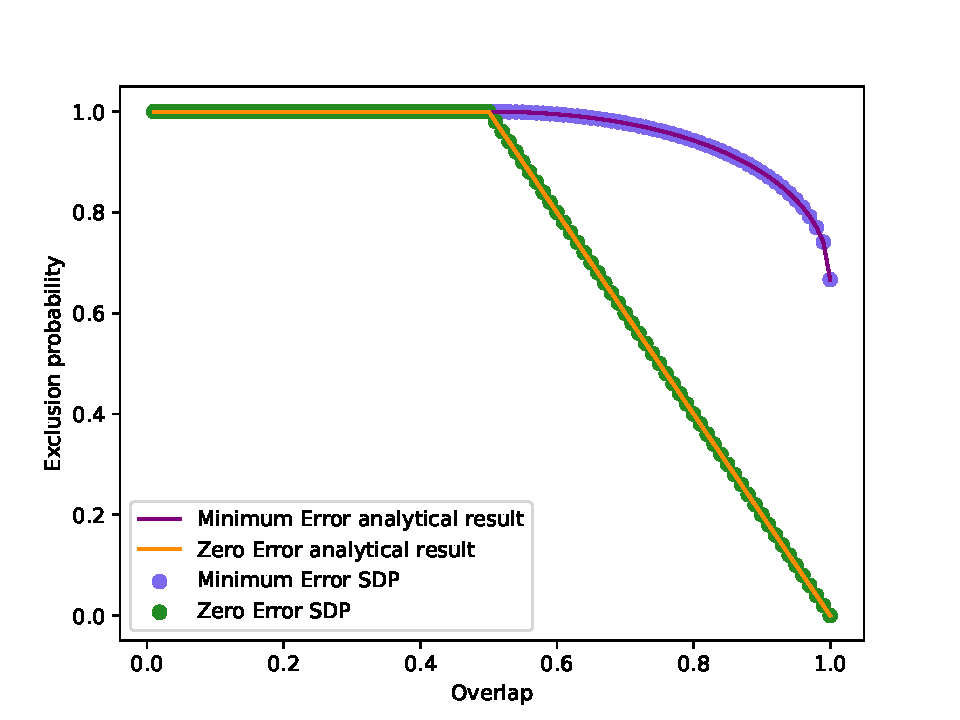
\includegraphics[width=0.49\textwidth]{../Plots/ExclusionOverlapVSSucessProbabilitySDPvsSRMZnOverlap3Phase0.pdf}
	\caption{Plot of the successful exclusion probabilities for the \gls{sdp} results for the \gls{me}, \gls{ze} protocols in a $\mathbb{Z}/3\mathbb{Z}$ ensemble impossing phase=$0$ as well as the results given by the analytical expressions (left). Perfect exclusion zone for a $\mathbb{Z}/3\mathbb{Z}$ ensemble in terms of the overlap's modulus and phase (right).}
	%\caption{Perfect exclusion zone for a $\mathbb{Z}/3\mathbb{Z}$ ensemble in terms of the overlap's modulus and phase.}
	\label{FigureQSEMEZ3ZPerfectExclusion}
\end{figure}

Crucially, we observe perfect exclusion is possible even when perfect discrimination is not \footnote{See section Comparison \gls{qsd} VS. \gls{qse} (\ref{appendixComparisonQSDvsQSE})}, in this regime seems to correspond to the ensembles such that the modulus of the overlap between two ensembles do not overtakes $\frac{1}{2}$. Nevertheless, this description is purely observational, we will give a better description in Section (\ref{sectionPerfectExclusionRegimeAndGeneralEnsembles}). In Figure (\ref{FigureQSEMEZ3ZPerfectExclusion}) (left) we highlight the regions where perfect exclusion is achieved, i.e. the red zone, even outside the perfect discrimination regime. Notice this regime appears in both protocols \gls{ze} and \gls{me}.

In Figure (\ref{FigureQSEMEZ3ZPerfectExclusion}) (right) we present de dependency on the modulus of the overlap in the $\mathbb{Z}/3\mathbb{Z}$ group-generated ensemble impossing the phase being equal to 0. The result is analogous to Figure (\ref{FigureQSDMEZESRM}) but in the exclusion task. The existence of the perfect exclusion zone appears in overlap values between 0 and $\frac{1}{2}$. 

%\begin{figure}[H]
%	\centering
%	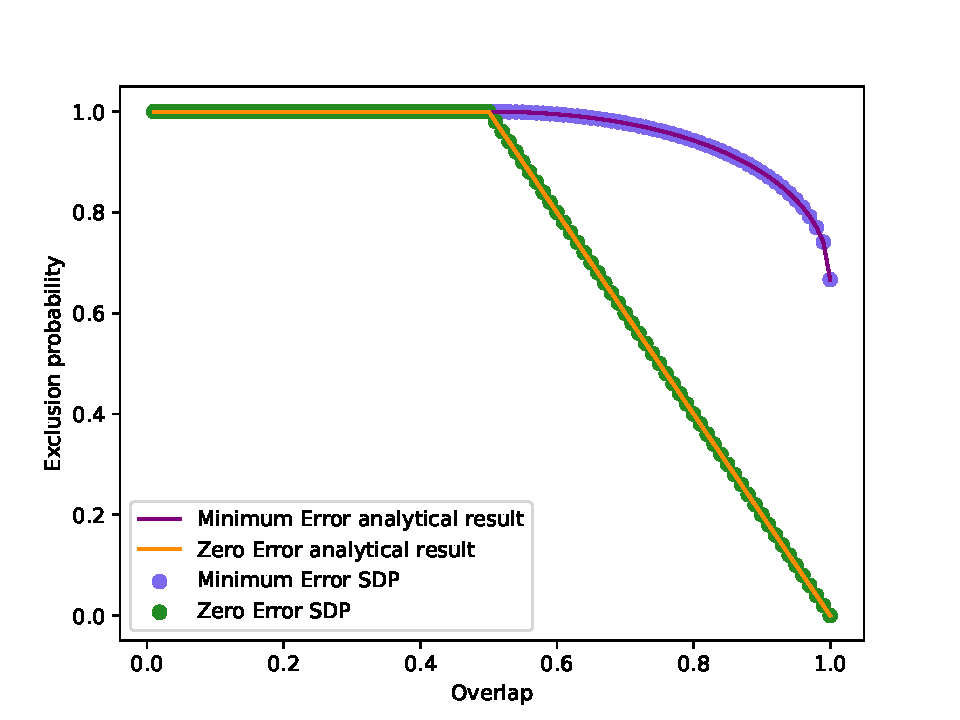
\includegraphics[width=0.49\textwidth]{../Plots/ExclusionOverlapVSSucessProbabilitySDPvsSRMZnOverlap3Phase0.pdf}
%	\caption{Plot of the successful exclusion probabilities for the \gls{sdp} results for the \gls{me}, \gls{ze} protocols in a $\mathbb{Z}/3\mathbb{Z}$ ensemble impossing phase=$0$ as well as the results given by the analytical expressions.}
%	\label{FigureQSEMEZESRM}
%\end{figure}

We highlight the good performance of the \gls{me} protocol up to limit values were the result tends to $\frac{2}{3}$ when the ensemble is made of indistingible states (i.e. the same state). 

\subsection{The perfect exclusion regime and general ensembles}\label{sectionPerfectExclusionRegimeAndGeneralEnsembles}

\hspace{20pt}In this section, we present the results for ensembles generated by the group $\mathbb{Z}/3\mathbb{Z}$, analyzed across the spectrum of eigenvalues, i.e. the analogus results from the previos section in the eigenvalues spectum. We also explicitly show the conditions for perfect exclusion, we give a proper analysis of this regime, and provide an initial exploration of the results for general ensembles being low bounded by the group-generated results of three quantum states.

Although the \emph{Overlap modulus - phase} spectrum might seem as the most intuituve representation, the spectrum of Gram's matrix eigenvalues results the most appropriate representation for the perfect exclusion zone as well as the discussion and its comparison for general ensembles. Carrying on with the previos discussion, one can check the two \gls{dof} now appear as two of the eigenvalues. In the Figure (\ref{FigureQSEMEZ3ZEigenValues}) the results for the exclusion task under the \gls{me} protocol (left) and \gls{ze} protocol (right) for the $\mathbb{Z}/3\mathbb{Z}$ group-generated ensemble are represented. The axis represent two of the eigenvalues of the Gram matrix and a heatmap presents the probability for a perfect exclusion in the given conditions.

\begin{figure}[H]
	\centering
	\begin{overpic}[width=0.49\textwidth, trim={2.3cm 0.8cm 4.4cm 2cm}, clip]{../Plots/ExclusionEignevaluesGroupGeneratedLowerBoundZ3.pdf}
	\put(20,25){\footnotesize{Perfect exclusion}}
	\put(50,50){$\mathcal{G}^{\mathbb{Z}/3\mathbb{Z}}<0$}
	\end{overpic}
	\begin{overpic}[width=0.49\textwidth, trim={2.3cm 0.8cm 4.4cm 2cm}, clip]{../Plots/ExclusionEignevaluesGroupGeneratedLowerBoundZ3ZeroError.pdf}
	\put(20,25){\footnotesize{Perfect exclusion}}
	\put(50,50){$\mathcal{G}^{\mathbb{Z}/3\mathbb{Z}}<0$}
	\end{overpic}
	\caption{Plot of the success exclusion probability in the eigenvalues spectrum for the \gls{me} (left) and \gls{ze} (right) protocol for a $\mathbb{Z}/3\mathbb{Z}$ group-generated ensemble.}
	\label{FigureQSEMEZ3ZEigenValues}
\end{figure}

The order in eigenvalues is obviated in the representation, i.e. we can find conditions such that $\lambda_i>\lambda_j$ and others conditions such that $\lambda_i<\lambda_j$ for $i,j\in\{1,2,3\}$

Notice the missing eigenvalue is determined by the other two via,\footnote{Recall we are factoring out the constant prior probability from the standard Gram Matrix, i.e. the actual eigenvalues from the Gram Matrix defined in Section \ref{sectionGramMatrixFormulation} are $\left\{\frac{\lambda_i}{3}\right\}_{i=1}^n$.}
\begin{align*}
	\lambda_3=3-\lambda_1-\lambda_2.
\end{align*}

Since the Gram matrix is a positive semidefinite matrix we know that $\lambda_3\geq0$, the limit case scenario $\lambda_3=0$ defines the line,
\begin{align*}
\lambda_2=3-\lambda_1,
\end{align*}

that constraints the possible eigenvalues to only reach values under this line. Otherwise the remaining value would be negative leading up to non-valid Gram matrices as discussed in the previos plots. Naturally, we also know $\lambda_1,\lambda_2>0$, then the region $\Omega$ where the system leads up to consistent Gram matrices is,
\begin{align*}
	\Omega=\left\{(\lambda_1,\lambda_2)\in\mathbb{R}^2\left|\lambda_1\geq0,\lambda_2\geq0,\lambda_1+\lambda_2\leq3\right.\right\}.
\end{align*}

This region $\Omega$ is depicted in the Figure (\ref{FigureQSEMEZ3ZEigenValues}) as boottom left triangle, where our system is recluded. Inside this region we can find the perfect exclusion zone, i.e. the eigenvalues such that Eq.(\ref{equationPerfectExclusionCondition}) is fulfilled. In particular, if we set $\lambda_i$ with $i\in\{1,2,3\}$ to be the greatest eigenvalues and denote $\lambda_j,\lambda_k$ as the remaining 2 eigenvalues, we know perfect exclusion to be archived if,
\begin{align*}
	\sqrt{\lambda_i}\leq \sqrt{\lambda_j}+\sqrt{\lambda_k}.
\end{align*}

With a little bit of algebra and recalling that $\lambda_3=3-\lambda_1-\lambda_2$ we can derive the regime of perfect exclusion denoted as $\Delta$ comprehends the eigenvalues such that,
\begin{align*}
	(\lambda_1,\lambda_2)\in \Delta\Leftrightarrow\lambda_1^2 + 4\lambda_2^2 + 4\lambda_1\lambda_2 - 12\lambda_1 - 12\lambda_2 + 9 \leq 0
\end{align*}

By plotting the $\Delta$ regio it turns out inmediatly this region corresponds to the colorless perfect exclusion regime in Figure (\ref{FigureQSEMEZ3ZEigenValues}).

%Figure (\ref{FigurePerfectExclusionZ3Z}) shows the $\Delta$ region. 
%\begin{figure}[H]
%	\centering
%	\begin{overpic}[width=0.5\textwidth, trim={1.8cm 0.8cm 2cm 2cm}, clip]{GeneralSources/PerfectExclusionZoneZ3Z.pdf}
%	\end{overpic}
%	\caption{Plot of the $\Delta$ region.}
%	\label{FigurePerfectExclusionZ3Z}
%\end{figure}

Naturally we can prove the perfect exclusion zone to be a subset of valid Gram matrixes i.e. $\Delta\subset \Omega$. Then, the non-perfect exclusion regime is the remaining part of the triangle i.e.,
\begin{align*}
	\text{Non-perfect exclusion regime}=\Omega\setminus \Delta.
\end{align*}

The limit case scenarios corresponding to $\lambda_i=3$ and $\lambda_j,\lambda_k=0$ are located in the vertex of the triangle\footnote{Remember this case correspond to sets with the same state repeated 3 times discussed in Section (\ref{sectionLimitCaseScenarios})}. Additionally, the cases corresponding to the edges are those with one state repeated 2 times and one different from the other 2. This ensembles can also be underestood as a limit case scenario systems.

In practice this scenario is entirely equivalent to a 2 quantum states exclusion (\gls{qse}) system. Nevertheless we know this to be equivalent to a 2 quantum states discrimination system (\gls{qsd}), therefore perfect discrimination/exclusion cannot be archived unless the states are orthogonal. This last case corresponds to the intersection of the elipse $\Delta$ with the triangles edges, this can be described as the ensembles with associated Gram matrices whose eigenvalues $\lambda_i,\lambda_j,\lambda_k$ are,
\begin{align*}
	\lambda_i=\lambda_j=\frac{3}{2}\quad\lambda_k=0.
\end{align*}

Additionally, we observe that no ensembles seem to have a lower exclusion success probability $P_{\gls{me}}^s$ under $\frac{2}{3}$ as expected from the discussion in Section (\ref{sectionLimitCaseScenarios}).

% Hence the results for the \gls{ze} protocol in \gls{qse} for a $\mathbb{Z}/3\mathbb{Z}$ ensemble are presented in Figure (\ref{FigureQSEZEZ3ZEigenValues}).


%\begin{figure}[H]
%	\centering
%	\begin{overpic}[width=0.75\textwidth, trim={2.3cm 0.8cm 4.4cm 2cm}, clip]{../Plots/ExclusionEignevaluesGroupGeneratedLowerBoundZ3ZeroError.pdf}
%		\put(20,25){\footnotesize{Perfect exclusion}}
%		\put(50,50){$\mathcal{G}^{\mathbb{Z}/3\mathbb{Z}}<0$}
%	\end{overpic}
%	\caption{Plot of the success exclusion probability in the eigenvalues spectrum for the \gls{ze} protocol for a $\mathbb{Z}/3\mathbb{Z}$ group-generated ensemble.}
%	\label{FigureQSEZEZ3ZEigenValues}
%\end{figure}

Regarding the \gls{ze} protocol result, i.e. Figure (\ref{FigureQSEMEZ3ZEigenValues}) right, we observe the result is consistent with all the previos observations and we can also observe the worst case scenario to tend to a 0 successfull exclusion probability as expected. Also, the probabilities remain with lower values than the ones obtained with the Minimum Error (\gls{me}) protocol. Still the perfect exclusion regions are the same.

Hence, we present the result for randomly generated ensembles, i.e. a general ensembles  in Figure (\ref{FigureQSEMEGenericEigenValues}).

\begin{figure}[H]
	\centering
	\begin{overpic}[width=0.59\textwidth, trim={2.3cm 0.8cm 4.4cm 2cm}, clip]{../Plots/ExclusionEignevalueRandom3.pdf}
		\put(20,25){\footnotesize{Perfect exclusion}}
		\put(50,50){$\mathcal{G}^{\mathbb{Z}/3\mathbb{Z}}<0$}
	\end{overpic}
	\begin{overpic}[width=0.39\textwidth, trim={6.5cm 2cm 4.4cm 2cm}, clip]{../Plots/ExclusionEignevalueRandom33D.pdf}
	\end{overpic}
	\caption{Heat map plot of the success exclusion probability in the eigenvalues spectrum for the \gls{me} protocol for a generic ensemble (left) and 3D Plot of the success exclusion probability in the eigenvalues spectrum for the \gls{me} protocol for a group-generated and generic ensembles (right)}
	\label{FigureQSEMEGenericEigenValues}
\end{figure}


A remarcable feature is that each ensemble has been checked to not have a successful exclusion probability that overtakes the value from the $\mathbb{Z}/3\mathbb{Z}$ group-generated ensemble pointing this value to be a lower bound for the general case scenario.


%\begin{figure}[H]
%	\centering
%	\caption{3D Plot of the success exclusion probability in the eigenvalues spectrum for the \gls{me} protocol for a group-generated and generic ensembles.}
%	\label{FigureQSEMEGenericEigenValues3D}
%\end{figure}

In Figure (\ref{FigureQSEMEGenericEigenValues}) we present a 3D plot for the comparison of the success probability for exclusion for ensembles of 3 states between generic and group-generated ensembles. The $x$ and $y$ axis representing de eigenvalues of the Gram matrix are analogous to previous figures. Nevertheless the $z$ axis shows the success probability for exclusion instead of the previous heat maps. Here we can observe how the randomly generated states raise the probabilities over the group-generated values. The generation of unitary matrices that fill $U(n)$ according Haar measure ensures the Gram matrices we are generating comprehend the entire set of possible Gram matrices homogeneously. Furthermore, we observe how the group-generated results lay under the results for general ensembles \gls{sdp}s, i.e. this results are bounded by the group-generated results.

\subsection{Distribution of the general ensembles success exclusion probability}

\hspace{20pt}In this section, we present the main results of the project. Specifically, we provide analytical results for generic ensembles and examine how the success probabilities for quantum state exclusion are distributed in relation to the lower bound defined by group-generated ensembles.

We begin by recalling that any Gram matrix $ \mathcal{G} $ can be decomposed as $ \mathcal{G} = U D U^\dagger $, where $ D $ is a diagonal matrix containing the eigenvalues $\{g_i\geq0\}_{i=1}^n $. We fix these eigenvalues such that
\begin{align*}
\sum_{i=1}^n g_i = 1,
\end{align*}
ensuring they are normalized.\footnote{Note that this eigenvalue notation differs from that used earlier in the document, where the eigenvalues of the Gram matrix were considered with an overall normalization factor of \( \frac{1}{n} \), assuming equal prior probabilities and were normalised to $n$. To avoid confusion, we change the notation for normalised eigenvalues that sum up to 1 for the general prior probabilities case.}

With this eigenvalue spectrum, we compute the analytical lower bound introduced in Section~\ref{sectionPreviousResults} and determine whether it falls within the perfect exclusion region. If it does, then any Gram matrix generated as $ \mathcal{G} = U D U^\dagger $ represents an ensemble for which perfect exclusion is feasible, and the lower bound is in fact the success probability, i.e. both are 1. Conversely, if the lower bound lies outside the perfect exclusion region, we explore different unitary matrices $ U $ to generate alternative Gram matrices that share the same eigenvalues, thus preserving the lower bound, while corresponding to distinct ensembles.

We use the algorithm proposed in~\cite{UnitaryMatricesGeneration} to generate unitary matrices sampled uniformly from \( U(n) \). This ensures a comprehensive exploration of the space of possible Gram matrices, i.e., ensembles, corresponding to a fixed lower bound.

It is important to highlight that this method also implicitly generates random prior probabilities for each state, since the diagonal elements of the Gram matrix are the priors probabilities, and generally will differ from one to another. Nevertheless, the analytical lower bound remains valid, as we will show in the following results.

\begin{figure}[H]
	\centering
	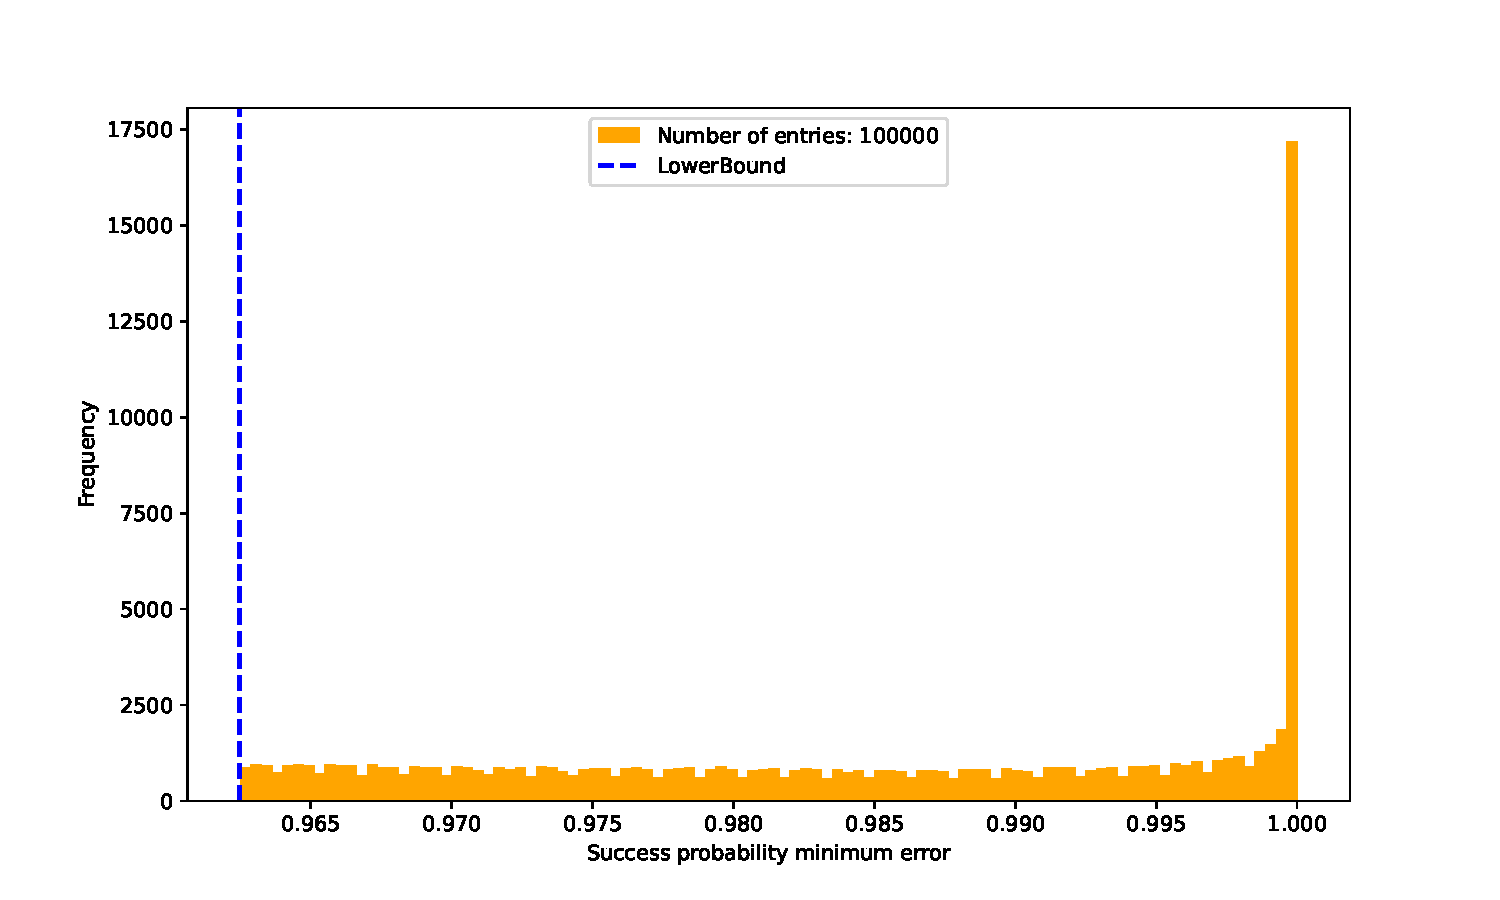
\includegraphics[width=0.75\textwidth, trim={1.0cm 0.3cm 2.4cm 1.5cm}, clip]{../Plots/ExclusionMinimumErrorRandomDistributionZ3Prob0.962.pdf}
	\caption{Hisotgram depicting the distribution of generated Gram Matrices via the success probability for \gls{me} protocol with a lower bound of 0.962 for 5 states ensembles of random priors probabilities.}
	\label{FigureDistZ5ME0.962}
\end{figure}

Figure (\ref{FigureDistZ5ME0.962}) shows the distribution of success probabilities for quantum state exclusion using the \gls{me} protocol computed via semidefinite programming (\gls{sdp}) for 5 states ensembles and random priors probabilities. The histogram's $x$-axis represents the exclusion success probability, while the $y$-axis indicates the frequency of occurrence across sampled ensembles. Additionally the dashed blue line marks the analytical lower bound.

We emphasize that each computed result has been verified not to fall below this analytical lower bound. Although a few discrepancies were observed, these occurred only at the fifth decimal place, where numerical precision limitations in the \gls{sdp} solver can affect reliability. These cases are treated as inconclusive due to numerical problems, and no inconsistencies have been found exceeding a deviation in the fourth decimal.

From the results in Figure (\ref{FigureDistZ5ME0.962}), we observe the ensembles are broadly distributed across a range of success probabilities. However, a significant clustering occurs near a success probability of 1 under the \gls{me} protocol, indicating that perfect exclusion is achievable for a substantial subset of these randomly generated ensembles.

These ensembles were generated uniformly by sampling unitary matrices $ U $ from $U(n)$, which determine the Gram matrices via the decomposition $\mathcal{G} = U D U^\dagger$. Ensembles with Gram matrices structurally similar to those of group-generated ensembles, particularly those diagonalized in the Fourier basis\footnote{Recall that we are working with ensembles of a prime number of states, for which the only known analytical result corresponds to the Gram matrix generated by $\mathbb{Z}/n\mathbb{Z}$, which is diagonalized in the Fourier basis. A more complete study would consider other group-generated cases.}, yield lower success probabilities. 

Interestingly, there exists a threshold of deviation from the Fourier basis beyond which all ensembles yield a success probability of 1. In other words, beyond a certain \emph{distance} from the group-generated case, i.e. the Fourier basis, the ensembles become sufficiently distinguishable to allow perfect exclusion, regardless of the specific basis in which their Gram matrices are diagonalised.

At this stage we can observe the crucial importance of the generation of the unitary matrices uniformly covering  $U(n)$, i.e. being generated according to the Haar measure. If we could not ensure we are exploring all the possible ensembles this observations and the study of the generic ensembles case would be completely pointless since we can overrepresent one specific kind of ensambles respect to others.

In Figure (\ref{FigureDistZ5ZE0.5}) we present the analogous results for the \gls{ze} protocol for ensembles consisting in 5 states with eigenvalues that lead to an analytical lower bound for success probability of $0.5$ in this protocol.

\begin{figure}[H]
	\centering
	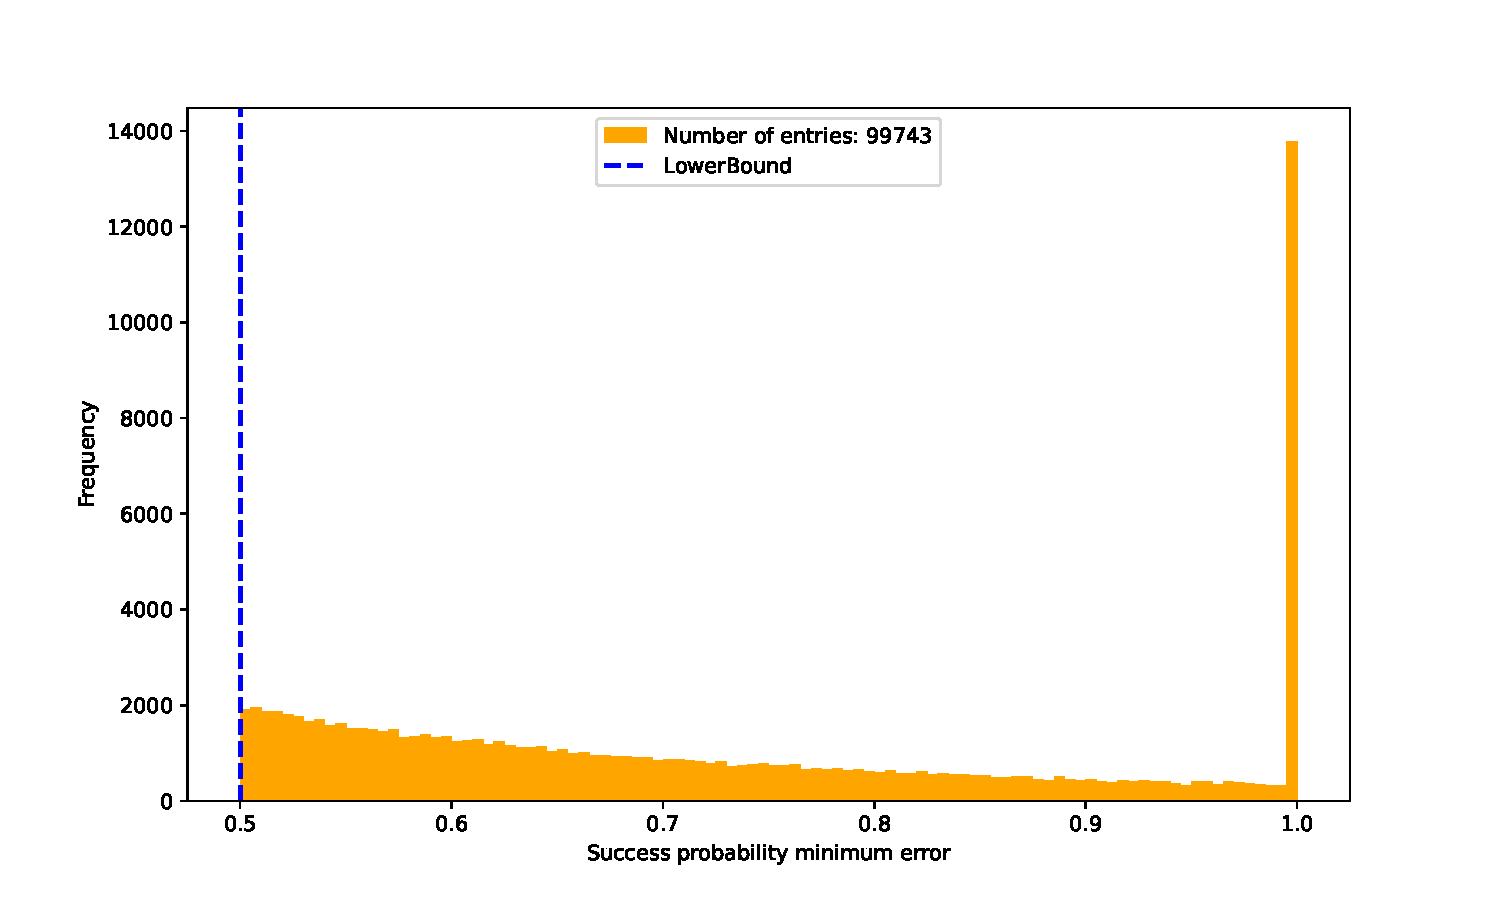
\includegraphics[width=0.75\textwidth, trim={1.0cm 0.3cm 2.4cm 1.5cm}, clip]{../Plots/ExclusionZeroErrorRandomDistributionZ3Prob0.5.pdf}
	\caption{Hisotgram depicting the distribution of generated Gram Matrices via the success probability for \gls{ze} protocol with a lower bound of 0.5 for 5 states ensembles of random priors probabilities.}
	\label{FigureDistZ5ZE0.5}
\end{figure}

Thus, we observe a similar behaviour respect to Figure (\ref{FigureDistZ5ME0.962}), still we attribute the pick of ensembles where perfect exclusion is feasible to the threshold of the \emph{distance} from the group generated case as previously discussed. Still some remarkable aspect of this protocol is the constant is the constant decay in the frequency for higher exclusion probabilities.

As before, no ensembles yields lower success exclusion probabilities than the lower bound, proving this as a lower bound of the generic case scenario.

\begin{figure}[H]
	\centering
	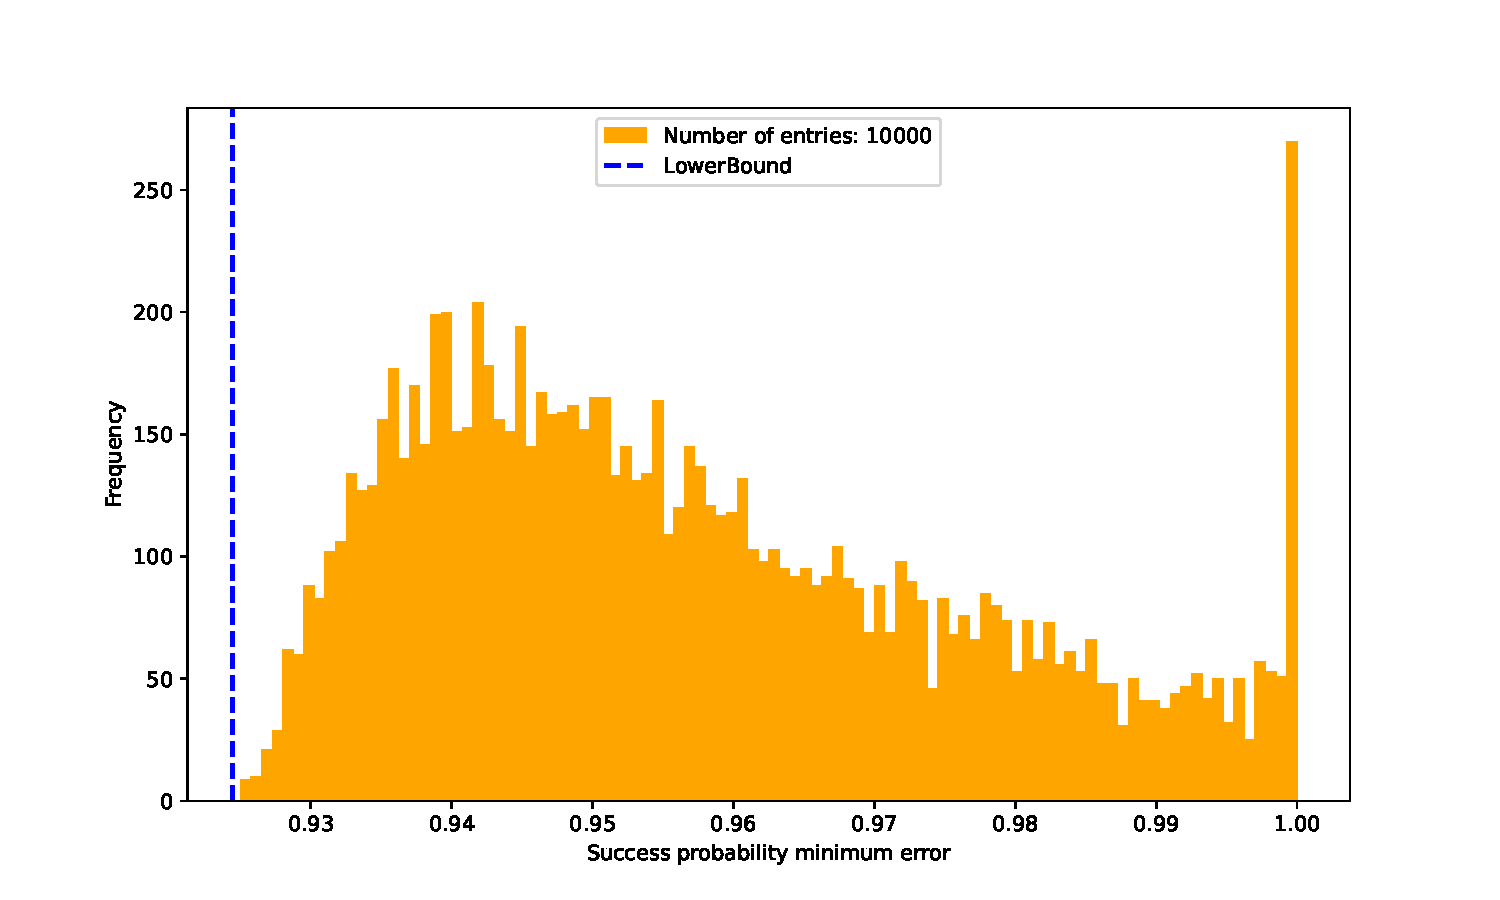
\includegraphics[width=0.49\textwidth, trim={1.0cm 0.3cm 2.4cm 1.5cm}, clip]{../Plots/ExclusionMinimumErrorRandomDistributionZ7Prob0.924.pdf}
	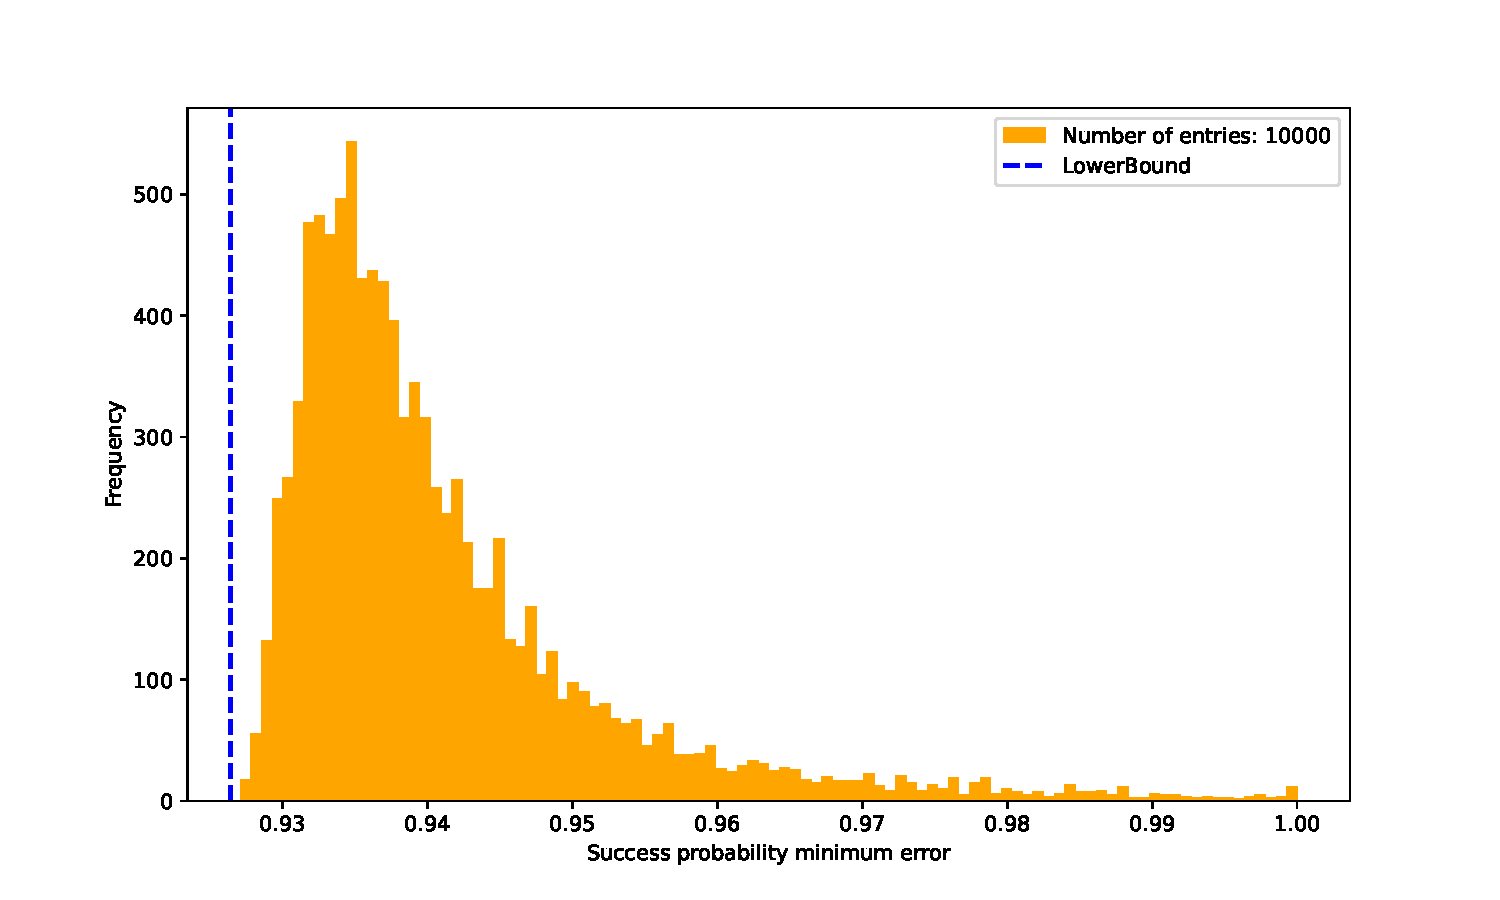
\includegraphics[width=0.49\textwidth, trim={1.0cm 0.3cm 2.4cm 1.5cm}, clip]{../Plots/ExclusionMinimumErrorRandomDistributionZ11Prob0.926.pdf}
	\caption{Hisotgram depicting the distribution of generated Gram Matrices via the success probability for \gls{me} protocol with a lower bound of 0.926 for 7 states (left) and 11 states (right) ensembles of random priors probabilities.}
	\label{FigureDistZ7Z11}
\end{figure}
In Figure~\ref{FigureDistZ7Z11}, we present the corresponding results for the \gls{me} protocol applied to ensembles composed of 7 (left) and 11 (right) quantum states, with a lower bound on the success exclusion probability of 0.926. As the number of states increases, the distribution approaches a Landau shape \cite{landau}. For ensembles of 7 elements, we still observe the phenomenon of accumulation near the perfect exclusion region. However, in the case of 11 states, only a small fraction of ensembles reach the perfect exclusion regime since the peak of the distribution is more narrow and the ensembles tend to agglomerate exclusion probabilities arround this peak.


\subsection{Intuition behind the results}

\hspace{20pt}The intuition behind the exclusion task for group-generated ensembles being the worst case scenario for this task, thus yielding a lower bound for the probability of excluding a hypothesis state in the general case is as follows. Consider an ensemble $\{\ket{\psi_i}\}_{i=1}^n$ with a certain degree of symmetry, and a state $\ket{\psi_j}$ known to be a member of this ensemble. Our goal is to perform the exclusion task, i.e., to identify a state $\ket{\psi_k} \in \{\ket{\psi_i}\}_{i=1}^n$ such that we \emph{suspect} $\ket{\psi_k} \neq \ket{\psi_j}$\footnote{We emphasize the word \emph{suspect} because in many scenarios we are not certain about $\ket{\psi_k} \neq \ket{\psi_j}$, which corresponds to the \emph{non-perfect exclusion} case.}.

Due to the symmetric nature of the ensemble, the states are very similar to each other. This makes it especially difficult to identify which state is different from the unknown state. In contrast, if the ensemble includes a state $\ket{\tilde{\psi}}$ that is very different from the others, it becomes easier to determine whether $\ket{\tilde{\psi}}$ matches the unknown state or not. Thus, when the symmetry is broken, exclusion can be performed more accurately.

To illustrate this more concretely, consider the following ensemble involving qubit states,
\begin{align}
\{\ket{\textcolor{red}{\uparrow}}, \ket{\textcolor{blue}{\uparrow}}, \ket{\textcolor{green}{\uparrow}}\}.
\end{align}

These are represented on a Bloch circle\footnote{The Bloch circle is a projection of the Bloch sphere onto a plane.} in Figure (\ref{FigureIntuitionExample}).

\begin{figure}[H]
	\centering
	\begin{tikzpicture}[scale = 1]
	\draw[thick] (0,0) circle(1cm);
  	\draw[line width=1.5pt,->,>=stealth, red] (0,0) -- (0,1);
  	\draw[line width=1.5pt,->,>=stealth, blue] (0,0) -- (0.17365,-0.9848);
  	\draw[line width=1.5pt,->,>=stealth, green] (0,0) -- (-0.17365,-0.9848);
	\end{tikzpicture}
	\caption{Representation of the ensemble states as projections on the Bloch circle.}
	\label{FigureIntuitionExample}
\end{figure}

It is evident that $\ket{\textcolor{red}{\uparrow}}$ is noticeably different from the other two states. The red arrow points in the opposite direction to the blue and green arrows. Therefore, given an unknown state $\ket{\uparrow}$ from this ensemble, it is relatively easy to determine whether $\ket{\uparrow} = \ket{\textcolor{red}{\uparrow}}$ or $\ket{\uparrow} \neq \ket{\textcolor{red}{\uparrow}}$. If $\ket{\uparrow} = \ket{\textcolor{red}{\uparrow}}$, we can exclude either $\ket{\textcolor{blue}{\uparrow}}$ or $\ket{\textcolor{green}{\uparrow}}$, otherwise, we can exclude $\ket{\textcolor{red}{\uparrow}}$. In both cases, the exclusion is straightforward.

This is closely related to the task of quantum state discrimination (\gls{qsd}). If $\ket{\uparrow} = \ket{\textcolor{red}{\uparrow}}$, the exclusion and discrimination tasks are practically equivalent. However, if $\ket{\uparrow} \neq \ket{\textcolor{red}{\uparrow}}$, it becomes very difficult to determine whether $\ket{\uparrow} = \ket{\textcolor{blue}{\uparrow}}$ or $\ket{\uparrow} = \ket{\textcolor{green}{\uparrow}}$, as these states are almost indistinguishable. Thus, in this ensemble, the exclusion task may be more feasible than discrimination, showcasing its strength in certain scenarios.

For a more analytical result, and regarding previos results in section (\ref{sectionPerfectExclusionRegimeAndGeneralEnsembles}), the success probability of this ensemble would be represented as a dot close to an edge of the triangle of Figure (\ref{FigureQSEMEGenericEigenValues}).
%From an analytical perspective, consider the Gram matrix $\mathcal{G}$ for this ensemble. We have,
%\\begin{align*}
%\braket{\textcolor{blue}{\uparrow}|\textcolor{red}{\uparrow}} \approx \braket{\textcolor{green}{\uparrow}|\textcolor{red}{\uparrow}} = \epsilon, \quad \braket{\textcolor{blue}{\uparrow}|\textcolor{green}{\uparrow}} = 1 - \epsilon, \quad \text{with } |\epsilon|^2 \approx 0.
%\end{align*}
%The states are normalized, so,
%\begin{align*}
%\braket{\textcolor{red}{\uparrow}|\textcolor{red}{\uparrow}} = \braket{\textcolor{blue}{\uparrow}|\textcolor{blue}{\uparrow}} = \braket{\textcolor{green}{\uparrow}|\textcolor{green}{\uparrow}} = 1.
%\end{align*}
%Hence, the Gram matrix is approximately,
%\begin{align*}
%\mathcal{G} = 
%\begin{pmatrix}
%1 & \epsilon & \epsilon^* \\
%\epsilon^* & 1 & 1 - \epsilon \\
%\epsilon & 1 - \epsilon^* & 1
%\end{pmatrix}.
%\end{align*}
%Neglecting terms of order $\epsilon^2$, the eigenvalues of $\mathcal{G}$ are approximately,
%\begin{align*}
%\{2 + \Re(\epsilon), 1, -2\Re(\epsilon)\}.
%\end{align*}

Now contrast this with a symmetric ensemble, as shown in Figure (\ref{FigureIntuitionExample2}).

\begin{figure}[H]
	\centering
	\begin{tikzpicture}[scale = 1]
	\draw[thick] (0,0) circle(1cm);
  	\draw[line width=1.5pt,->,>=stealth, red] (0,0) -- (0,1);
  	\draw[line width=1.5pt,->,>=stealth, blue] (0,0) -- (0.866,-0.5);
  	\draw[line width=1.5pt,->,>=stealth, green] (0,0) -- (-0.866,-0.5);
	\end{tikzpicture}
	\caption{Symmetric ensemble represented on the Bloch circle.}
	\label{FigureIntuitionExample2}
\end{figure}

This configuration exhibits perfect symmetry. Define a unitary operator $\mathcal{U}$ such that,
\begin{align*}
\mathcal{U} \ket{\textcolor{red}{\uparrow}} = \ket{\textcolor{blue}{\uparrow}},
\end{align*}
then by symmetry,
\begin{align*}
\mathcal{U} \ket{\textcolor{blue}{\uparrow}} = \ket{\textcolor{green}{\uparrow}}, \quad \mathcal{U} \ket{\textcolor{green}{\uparrow}} = \ket{\textcolor{red}{\uparrow}}.
\end{align*}
Hence,
\begin{align*}
\mathcal{U}^3 = \mathds{1}|_{\text{Bloch circle}},
\end{align*}
where $\mathds{1}|_{\text{Bloch circle}}$ denotes the identity operator restricted to this subspace. This implies the ensemble is generated by a cyclic group of order 3, i.e., $\mathbb{Z}/3\mathbb{Z}$.

In such a group-generated ensemble, distinguishing any pair of states is equally difficult due to symmetry. Therefore, exclusion becomes more challenging, representing a worst-case scenario compared to the asymmetric case.

\newpage
\section{Conclusions}

\hspace{20pt}We have presented a robust protocol for generating ensembles of quantum states, along with their corresponding prior probabilities, in a manner that uniformly samples the full space of possible ensembles. This approach ensures a comprehensive and unbiased exploration for the study of Quantum State Exclusion (\gls{qse}). Using this ensemble generation method, we have computed the corresponding Semidefinite Programming (\gls{sdp}) optimization problems, allowing us to numerically verify and support the analytical results obtained for the success and error probabilities associated with group-generated ensembles.

The analytical results, presented in Section~\ref{sectionPreviousResults} \emph{Previous Results}, for the success probability in Quantum State Exclusion (\gls{qse}) for the Minimum Error (\gls{me}) and Zero Error (\gls{ze}) protocols for equal prior probabilities for group-generated ensambles have provide lower bounds for the success probability in Quantum State Exclusion (\gls{qse}) the same protocols. Our numerical simulations confirm that these group-generated ensembles consistently achieve the lowest exclusion success probabilities, thus validating their role as theoretical lower bounds when compared to the broader set of randomly generated ensembles. We have also offered conceptual insights into the intuition of why these bounds persist in the general case, including a geometric interpretation based on Gram matrix structure and ensemble distinguishability.

In addition, we have explored in detail the specific case of the cyclic group $\mathbb{Z}/3\mathbb{Z}$, the only group-generated ensemble that can be faithfully represented in two dimensions. This visualization not only has provided intuition but also demonstrates the practical advantage of \gls{qse} over its counterpart, Quantum State Discrimination (\gls{qsd}). These results strengthen the case for employing \gls{qse} in quantum information tasks where conventional discrimination strategies fall short.

The observations made in this project open the door to further analytical and numerical investigations. Extending this analysis to more generic ensembles, that may reveal new structural properties and exclusion capabilities. Furthermore, from the results and discussions in this project it results obvious that research in hybrid protocols that interpolate between Minimum Error \gls{me} and Zero Error \gls{ze} protocols as well as \gls{qse} and \gls{qsd} could potentially yield more optimal performance in practical applications.

In summary, this work contributes both rigorous numerical evidence and conceptual motivation for viewing group-generated ensembles as the worst case scenario in the study of quantum state exclusion, i.e. leading up to a lower bound in the exclusion probability. It also highlights promising directions for future work, including the development of tighter bounds, hybrid exclusion strategies, and generalizations of the analitical results.

%%%%%%%%%%%%%%%%%%%%%%%%%%%%%%%%%%%%%%%%%%
%%%%%%%%%%%%%%%% BIBLIOGRAPHY %%%%%%%%%%%%%%%%%
%%%%%%%%%%%%%%%%%%%%%%%%%%%%%%%%%%%%%%%%%%
\newpage
\bibliographystyle{plain}
\bibliography{references} 
%%%%%%%%
\section*{List of abbreviations}
\renewcommand{\glsnamefont}[1]{\textbf{#1}}
\printnoidxglossary[type=main, title={\vspace{-1cm}}, nonumberlist, nogroupskip, style=super]

\section*{Acknowledgements}

\hspace{20pt}I am grateful to Dr. Ramón Muñoz Tapia for allowing me to be one of his pupils and for presenting this project. I am also deeply grateful to PhD. student Santiago Llorens Fernández for being the lighthouse that illuminates my path throughout this journey.

I would like to acknowledge my mother and sister for their unconditional support, and my father for the values he taught me. Additionally, I would like to thank my friends Francisco Montaño, David Muñoz and Manel Martin for listening to my monologues about my excitement for Quantum State Exclusion.


\newpage
\appendix

\section{Dual Formulation of the Problem}\label{sectionDualFormulationOfTheProblem}

\hspace{20pt}It is often useful to consider the \emph{dual} version of a \gls{sdp} problem, as it provides both conceptual insights and practical advantages for verifying optimality. 

Consider the ensemble $\left\{ \left( \rho_i, \frac{1}{n} \right) \right\}_{i=1}^n$, where each state $\rho_i$ appears with uniform prior probability $1/n$. The dual SDP corresponding to the Minimum Error (\gls{me}) exclusion protocol, when expressed in terms of the error probability, is given by,
\begin{align*}
	\tilde{P}_{\gls{me}}^e = \max_{\Gamma} \quad & \tr{\Gamma} \\
	\text{subject to} \quad & \frac{\rho_i}{n} - \Gamma \geq 0 \quad \forall i \in \{1, \dots, n\}, \\
	& \Gamma^\dagger = \Gamma,
\end{align*}
where $\tilde{P}$ denotes the dual version of the problem.

Similarly, the dual SDP for the success probability in the same protocol reads,
\begin{align*}
	\tilde{P}_{\gls{me}}^s = \min_{\Gamma} \quad & 1 - \tr{\Gamma} \\
	\text{subject to} \quad & \frac{\rho_i}{n} - \Gamma \geq 0 \quad \forall i \in \{1, \dots, n\}, \\
	& \Gamma^\dagger = \Gamma.
\end{align*}

For the \gls{ze} protocol the dual version of the \gls{sdp} for the error probability is,
\begin{align*}
	\tilde{P}_{\gls{ze}}^s = \max_{X\geq 0} \quad & 1-\tr{X} \\
	\text{subject to} \quad & \sum_{g\in\mathcal{G}}U_gXU_g^\dagger+ \nu\ket{\psi}\bra{\psi}-\Omega \geq 0 \quad \nu \in \mathbb{R}.
\end{align*}

Hence the success probability is,

\begin{align*}
	\tilde{P}_{\gls{ze}}^s = \min_{X\geq 0} \quad & \tr{X} \\
	\text{subject to} \quad & \sum_{g\in\mathcal{G}}U_gXU_g^\dagger+ \nu\ket{\psi}\bra{\psi}-\Omega \geq 0 \quad \nu \in \mathbb{R}.
\end{align*}

One of the primary uses of the dual formulation is in establishing optimality. If a POVM ansatz yields equal objective values for both the primal and dual problems, i.e., $P = \tilde{P}$, then strong duality holds and the measurement is guaranteed to be optimal.

This duality principle not only provides a tool for verification but also suggests constructive approaches to discovering optimal measurements, especially in structured ensembles such as those generated by group actions.

\section{Computation of Gram Matrices for a group-generated ensembles}\label{appendixComputationGroupGeneratedGramMatrices}

\hspace{20pt}We can compute the Gram matrix for any group-generated ensemble by using the Cayley table~\cite{CayleyTable}, also known as the \emph{multiplication table}, of the group. For example, consider the smallest non-commutative group, $S_3$, consisting of the symmetries and rotations of an equilateral triangle. Denoting the identity as $e$, the rotations elements as $s$, $s^2$ (one being the result of 2 times the other) and the symmetries $p$, $q$, and $r$, the Cayley table is,
\begin{table}[H]
    \centering
    \caption{Cayley table of the $S_3$ group.}
    \label{tab:Cayley-S3}
    \setlength{\tabcolsep}{12pt}
    \renewcommand{\arraystretch}{1.3}
    \begin{tabular}{|>{\columncolor{gray!20}}c||c|c|c|c|c|c|}
        \hline
        \rowcolor{gray!20}
        $S_3$ & $e$ & $s$ & $s^2$ & $p$ & $q$ & $r$ \\
        \hline\hline
        $e$   & $e$ & $s$ & $s^2$ & $p$ & $q$ & $r$ \\
        $s^2$ & $s^2$ & $e$ & $s$ & $r$ & $p$ & $q$ \\
        $s$   & $s$ & $s^2$ & $e$ & $q$ & $r$ & $p$ \\
        $p$   & $p$ & $r$ & $q$ & $e$ & $s^2$ & $s$ \\
        $q$   & $q$ & $p$ & $r$ & $s$ & $e$ & $s^2$ \\
        $r$   & $r$ & $q$ & $p$ & $s^2$ & $s$ & $e$ \\
        \hline
    \end{tabular}
\end{table}

We now identify $S_3$ as a group of unitary matrices\footnote{We treat each group element as a unitary matrix, and the group operation as matrix multiplication.}. It follows that the Gram matrix of the $S_3$ group-generated ensemble is the matrix of expected values of the Cayley table entries with respect to the seed state $\ket{\psi}$. That is,
\begin{align*}
	\mathcal{G}^{S_3}_{\psi} = \frac{1}{6}\begin{pmatrix}
        1 & \braket{s}_\psi & \braket{s^2}_\psi & \braket{p}_\psi & \braket{q}_\psi & \braket{r}_\psi \\ 
        \braket{s^2}_\psi & 1 & \braket{s}_\psi & \braket{r}_\psi & \braket{p}_\psi & \braket{q}_\psi \\
        \braket{s}_\psi & \braket{s^2}_\psi & 1 & \braket{q}_\psi & \braket{r}_\psi & \braket{p}_\psi \\
        \braket{p}_\psi & \braket{r}_\psi & \braket{q}_\psi & 1 & \braket{s^2}_\psi & \braket{s}_\psi \\
        \braket{q}_\psi & \braket{p}_\psi & \braket{r}_\psi & \braket{s}_\psi & 1 & \braket{s^2}_\psi \\
        \braket{r}_\psi & \braket{q}_\psi & \braket{p}_\psi & \braket{s^2}_\psi & \braket{s}_\psi & 1
	\end{pmatrix}.
\end{align*}

Notice we have assumed equal prior probabilities, i.e. $\eta_i = \eta_j = \frac{1}{6}$. In the non-equal prior probabilities regime we only need to multiply each element for $\sqrt{\eta_i\eta_j}$ insted of $\frac{1}{6}$. Additionally, note that $\braket{e}_\psi = 1$ since $e = \mathds{1}$. Moreover, since $\mathcal{G}^{S_3}$ is Hermitian, we conclude,
\begin{align*}
\braket{p}_{\psi},\ \braket{q}_{\psi},\ \braket{r}_{\psi} \in \mathbb{R}, \quad \forall \ket{\psi} \in \mathcal{H},
\end{align*}

which implies the unitary matrices corresponding to the triangle symmetries $p$, $q$, and $r$ are Hermitian. As a matter of fact we know the eigenvalues of this matrices can only be $\pm 1$ and at least one of them must be $-1$.\footnote{Otherwise, they would be the identity and we know them to be different by construction.} This procedure generalizes to any finite group $G$, showing that computing the Cayley table is equivalent to computing the Gram matrix of the corresponding group-generated ensemble.

\section{Comparison \gls{qsd} vs. \gls{qse}}\label{appendixComparisonQSDvsQSE}

\hspace{20pt}Here we present the results for the Quantum State Discrimination (\gls{qsd}) task to motivate the problem and highlight contrasts with the Quantum State Exclusion (\gls{qse}) task, which is the focus of this study.

\begin{figure}[H]
	\centering
	\begin{overpic}[width=0.5\textwidth, trim={2.3cm 0.8cm 4.5cm 2cm}, clip]{../Plots/DiscriminationOverlapVSPhaseVSMinimumErrorProbabilityZ3HeatMap.pdf}
		\put(60,25){$\mathcal{G}^{\mathbb{Z}/3\mathbb{Z}}<0$}
		\put(60,55){$\mathcal{G}^{\mathbb{Z}/3\mathbb{Z}}<0$}
	\end{overpic}
	\caption{Heatmap of the success probability for minimum error (\gls{me}) quantum state discrimination for a $\mathbb{Z}/3\mathbb{Z}$ group-generated ensemble.}
	\label{FigureQSDMEZ3ZHeatmap}
\end{figure}

In these conditions, the \gls{srm}\footnote{Also known as the Pretty Good Measurement.} is optimal, i.e. the result of the \gls{sdp} matches the one obtained from the \gls{sdp} in \gls{me} protocol. In particular, the \gls{srm} is obtained from the square root decomposition of the Gram matrix,
\begin{align*}
	\mathcal{G} = S^\dagger S = S^2
\end{align*}

and is the standard in \gls{qsd} under the \gls{me} protocol \cite{OptimalitySRM}. From section (\ref{sectionGramMatrixFormulation}) we know the success probability for a successful discrimination with \gls{srm} reeds,
\begin{align*}
	P_{\gls{srm}}^s=\frac{1}{n}\sum_{i=0}^nS_{i,i}^2
\end{align*}

were $S_{i,i}$ denotes the diagonal elements of $S$ and $n$ the number of quantum states\footnote{In this case we are taking $n=3$.}.

As expected, no ensemble yields a success probability below $1/3$, consistent with the discussion in Section (\ref{sectionLimitCaseScenarios}). Moreover, as the modulus of the overlap approaches zero, the success probability approaches one, corresponding to orthogonal states, again matching expectations.

Figure (\ref{FigureQSDZEZ3ZHeatmap}) shows analogous results for the Zero Error (\gls{ze}) protocol under the same conditions.

\begin{figure}[H]
	\centering
	\begin{overpic}[width=0.5\textwidth, trim={2.3cm 0.8cm 4.5cm 2cm}, clip]{../Plots/DiscriminationOverlapVSPhaseVSSuccessProbabilityZeroErrorZ3HeatMap.pdf}
		\put(60,25){$\mathcal{G}^{\mathbb{Z}/3\mathbb{Z}}<0$}
		\put(60,55){$\mathcal{G}^{\mathbb{Z}/3\mathbb{Z}}<0$}
	\end{overpic}
	\caption{Heatmap of the success probability for zero-error (\gls{ze}) quantum state discrimination for a $\mathbb{Z}/3\mathbb{Z}$ group-generated ensemble.}
	\label{FigureQSDZEZ3ZHeatmap}
\end{figure}

Again, the ZE protocol yields lower probabilities due to its constraints and the limit case scenarios match with the previos discussion in Section (\ref{sectionLimitCaseScenarios}) and Section (\ref{sectionResultsAndDiscussion}). 

Figure (\ref{FigureQSDMEZESRM}) compares the performance of the ME, ZE, and SRM protocols.

\begin{figure}[H]
	\centering
	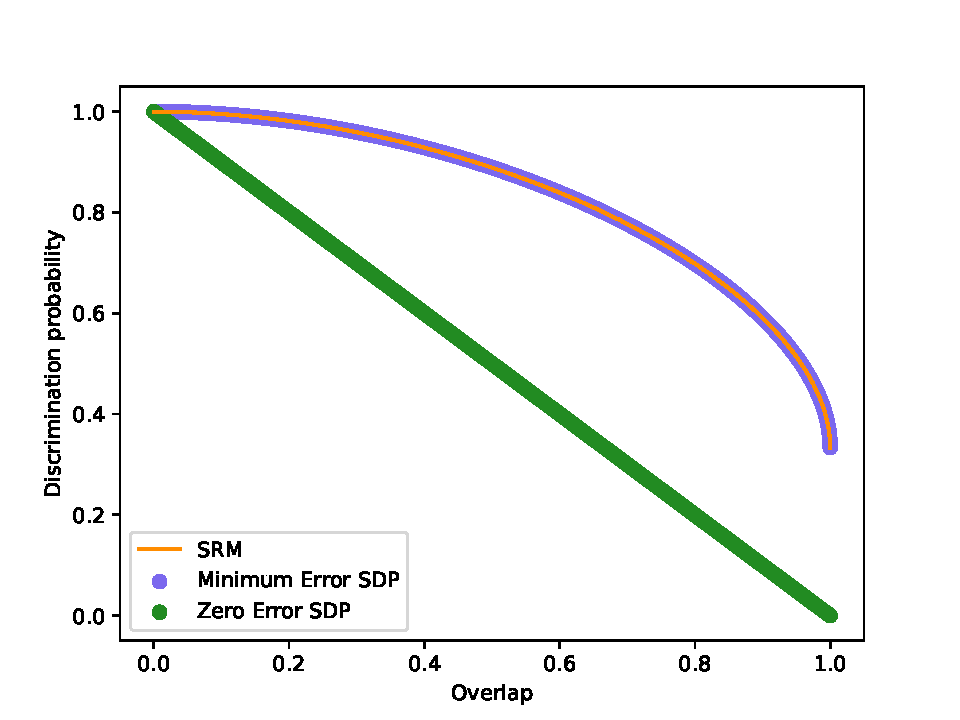
\includegraphics[width=0.5\textwidth]{../Plots/DiscriminationOverlapVSSucessProbabilitySDPvsSRMZnOverlap3Phase0.pdf}
	\caption{Comparison of successful discrimination probabilities for ME, ZE, and SRM protocols in a $\mathbb{Z}/3\mathbb{Z}$ ensemble impossing phase=$0$.}
	\label{FigureQSDMEZESRM}
\end{figure}

As expected, perfect discrimination is only achieved when the overlap is zero (orthogonal states), and the \gls{srm} success probability matches the one obtained from the numerical \gls{sdp}. 

Moreover, we observe the results in \gls{qse} are substancially better, the exclusion can be performed with higher precission than the discrimination. This observations is expected. Let us suppose we perform a correct guess in the discrimination of our unknown state, then if we know to which state is correlated our unknown state, we know which states is not correlated to, in other words
\begin{align*}
	\text{correct discrimination}\Rightarrow\text{correct exclusion}.
\end{align*}

However, let us suppose we perform a correct guess in the exclusion task, still we are ignoring which is our unknown state, then,
\begin{align*}
	\text{correct exclusion}\nRightarrow\text{correct discrimination}.
\end{align*}

Hence, archiving a correct outcome in the discrimination task implies a correct outcome in the exclusion task but the reciprocal is untrue. This trivial discussion explains the differences in the results and reinforces the potential of \gls{qse}.

This highlights the motivation behind the study of \gls{qse}, which allows for perfect exclusion in cases where discrimination is impossible. The possibility perfect exclusion for \gls{qse} is a major motivation for its study. For example, in a regime where perfect exclusion is possible, having access to multiple copies of a unknown state enables hybrid exclusion-discrimination protocols that can outperform purely discriminative strategies. Even partial information, such as the exclusion of a single quantum state, has value in certain quantum information theories. These features make \gls{qse} a fertile ground for further theoretical and applied research.

\section{Limit Case Scenarios}\label{sectionLimitCaseScenarios}

\hspace{20pt}Let us study the Gram matrix of a limit ensemble composed of $n$ identical quantum states with equal probabilities, i.e. the same state is repeated $n$ times in the ensemble with the same probability.\footnote{This case may appear paradoxical, since there is no way to distinguish between identical states. Nevertheless, we present it as a limiting scenario.} The Gram matrix reads:
\begin{align*}
	\mathcal{G}^{\text{limit}} = \frac{1}{n}\begin{pmatrix}
 1 & 1 & \cdots & 1 \\
 1 & 1 & \cdots & 1 \\
 \vdots & \vdots & \ddots & \vdots \\
 1 & 1 & \cdots & 1 \\
\end{pmatrix}.
\end{align*}

The eigenvalues of this matrix are:
\begin{align*}
	\lambda_n &= 1, \\
	\lambda_{n-1} &= 0, \\
	\vdots \\
	\lambda_1 &= 0.
\end{align*}

Clearly, this set of eigenvalues does not satisfy Eq. (\ref{equationPerfectExclusionCondition}), i.e., we are in the non-perfect exclusion regime. In fact, we can interpret this ensemble as a group-generated ensemble from the \emph{trivial group},\footnote{The trivial group is the group consisting solely of the neutral/identity element.} which generates no variation.

Thus, the success and error probabilities for both the \gls{me} protocol is,
\begin{align*}
	P_{\gls{me}}^e =& \frac{1}{n},\\
	P_{\gls{me}}^s =& \frac{n-1}{n}.
\end{align*}

The intuition behind this result is clear. If there is no physical way to distinguish between states, the exclusion must be made randomly, with uniform probability. This observation also extends naturally to \gls{qsd}.

Since this is a limiting case scenario, the success probability for \gls{qse} must be strictly greater than $\frac{n-1}{n}$ (i.e., the error probability must be less than $\frac{1}{n}$) and for \gls{qsd} the success probabilities must be strictly greater than $\frac{1}{n}$ (i.e., the error probability must be less than $\frac{n-1}{n}$)\footnote{In this case scenario the discrimination task is the counterpart of the exclusion task.}. Notice this result holds only for the \gls{me} protocol. Otherwise, since the exclusion cannot be accomplished without ambiguity, the successfull exclusion probability for the \gls{ze} protocol is 0 for either \gls{qse} or \gls{qsd} (i.e., the error exclusion probability is 1), 
\begin{align*}
	P_{\gls{ze}}^e =& 1,\\
	P_{\gls{ze}}^s =& 0.
\end{align*}

The opposite limiting case is an ensemble of $n$ orthogonal quantum states $\{\rho_i\}_{i=1}^{n}$. In this case, the Gram matrix becomes the identity,
\begin{align*}
	\mathcal{G} = \mathds{1}.
\end{align*}

Under these conditions, both \gls{qse} and \gls{qsd} are trivial, as the states form an orthonormal basis. In particular, in the space spanned by these states, we have,
\begin{align*}
	\sum_{i=1}^{n} \rho_i = \mathds{1},
\end{align*}

which means that the set $\{\rho_i\}$ is itself a \gls{povm}. The measurement corresponding to this \gls{povm} allows perfect identification, or exclusion, hence both \gls{qse} and \gls{qsd} can be performed without error.

\end{document}
